% P9: Peripheral Conservatism as Archaeological Proxy
% Target: JSEAS (NUS Press) — Chicago footnotes, 9,000-12,000 words
% Compile: pdflatex → biber → pdflatex → pdflatex

\documentclass[12pt,a4paper]{article}

% ============================================================
% Packages
% ============================================================
\usepackage[utf8]{inputenc}
\usepackage[T1]{fontenc}
\usepackage{mathptmx}  % Times New Roman equivalent
\usepackage[english]{babel}
\usepackage{csquotes}
\usepackage{setspace}
\doublespacing
\usepackage[left=2.5cm,right=2.5cm,top=2.5cm,bottom=2.5cm]{geometry}
\usepackage{graphicx}
\graphicspath{{figures/}}
\usepackage{amssymb}
\usepackage{booktabs}
\usepackage{longtable}
\usepackage{array}
\usepackage{url}
\usepackage{hyperref}
\hypersetup{colorlinks=true,linkcolor=black,citecolor=black,urlcolor=blue}

% Footnote-style citations (Chicago-like)
\usepackage[backend=biber,style=verbose-note,sorting=nty]{biblatex}
\addbibresource{references.bib}

% ============================================================
% Title
% ============================================================
\title{\textbf{Peripheral Conservatism as Archaeological Proxy: Linguistic, Ritual, and Botanical Evidence for a Pre-Hindu Nusantaran Substrate}}
\author{Mukhlis Amien\textsuperscript{1,*} \and Go Frendi Gunawan\textsuperscript{1}\\[6pt]
\small \textsuperscript{1}Lab Data Sains, Universitas Bhinneka Nusantara\\
\small \textsuperscript{*}Corresponding author. ORCID: 0000-0002-1848-167X}
\date{}

\begin{document}
\maketitle
\thispagestyle{empty}

% ============================================================
% Abstract (~200 words for JSEAS)
% ============================================================
\begin{abstract}
\noindent
Geographic and cultural peripheries in Nusantara preserve archaic layers overwritten in historical centres by Indianization, Islamization, and colonialism. This paper proposes the Peripheral Conservatism Framework (PCF), a systematic methodology for recovering pre-Hindu cultural substrates from three types of peripheral archive: geographic (island and highland isolates), political (zones outside court standardization), and temporal (communities exported before an overwriting event). The framework is demonstrated through three independent recovery channels: lexical conservation, mortuary ritual structure, and botanical burial practice.

Analysis of 210 basic vocabulary concepts from the Austronesian Basic Vocabulary Database (ABVD) reveals that Balinese retains 40.3\% Proto-Malayo-Polynesian (PMP) cognates versus 33.0\% for standard Javanese, with the peripheral advantage concentrated in nature-domain vocabulary (+27.2\%). Merina Malagasy (40.8\%) provides a dateable \textit{c.}~1200~CE calibration point. A critical botanical correction establishes that \textit{Plumeria} (kamboja), ubiquitous at Javanese cemeteries, is a post-1560 New World introduction; the genuine pan-Austronesian aromatic is \textit{Canarium}~spp. Screening of 268 Old Javanese inscriptions confirms the described civilization was overwhelmingly organic (63.4\% mention organic materials), while the Indianization itself proves non-permanent: Sanskrit vocabulary ratio declines from 0.807 (ninth century) to 0.569 (thirteenth century). Together, these findings support the PCF as a methodology for recovering invisible cultural substrates from living peripheral communities rather than from archaeological excavation at overwritten centres.
\end{abstract}

\newpage
\setcounter{page}{1}

% ============================================================
% 1. INTRODUCTION
% ============================================================
\section{Introduction: The Periphery as Archive}

\subsection{The Overwriting Problem}

Standard models of cultural diffusion assume that innovations originate at centres and spread outward. A corollary, less often stated, is that \emph{centres overwrite themselves}---the same prestige pressure that disseminates innovations also erases the strata beneath them.\footnote{For the general model, see the ``wave theory'' of linguistic diffusion in \autocite{blust1995austronesian}. The overwriting problem is analogous to palimpsest formation in manuscript studies: each new layer obscures the one beneath.} Peripheries, by definition, receive prestige innovations later, incompletely, or not at all. They are therefore not cultural backwaters but involuntary archives---preserving older strata precisely because they were never fully rewritten.

In Nusantara, three successive overwriting events have shaped the observable cultural record:

\begin{enumerate}
\item \textbf{Indianization} (\textit{c.}~400--1500~CE): Sanskrit cosmology, Hindu-Buddhist statecraft, cremation rites, caste-inflected speech registers, and a phonological inventory (33~consonants) imposed upon an Austronesian substrate of approximately 17~consonants.

\item \textbf{Islamization} (\textit{c.}~1200--1700~CE): Inhumation burial, Arabic loanwords into formal registers, dietary law, and the progressive erasure of Hindu-Buddhist iconography from public space. The process was neither uniform nor complete---Bali and pockets of East Java remained Hindu.

\item \textbf{Colonialism} (\textit{c.}~1600--1945~CE): Dutch administrative vocabulary, Christian burial in some regions, standardization of written Malay/Indonesian, and the imposition of European categories on indigenous knowledge systems. Colonial-era ethnography simultaneously recorded and distorted local practices.
\end{enumerate}

Each event added a new layer of vocabulary, cosmology, and material culture while partially obscuring the layer beneath. Communities that escaped the full force of these waves---by geography, resistance, or isolation---constitute the involuntary archives from which this paper proposes to recover pre-Hindu substrates.

\subsection{The Archaeological Blank}

In volcanic Java, the archival function of peripheral communities acquires special significance. The same volcanic processes that bury physical archaeological evidence at 2.4--6.2~mm/year\footnote{\autocite{amien2026a}. Five independent calibration points from two volcanic systems (Merapi, Kelud) yield a mean of 4.4~$\pm$~1.2~mm/year. At this rate, pre-400~CE sites lie at depths of 163--326~cm---well below the reach of conventional surface survey.} also accelerate the decomposition of organic materials that constituted the majority of pre-Hindu material culture (see~\S\ref{sec:organic}). The result is a compounding invisibility: physical evidence is destroyed from below by volcanism while cultural markers are overwritten from above by successive prestige waves.

This double erasure has produced what may be called the ``archaeological blank'' of pre-Hindu western Indonesia---the assumption, embedded in textbook narratives, that complex civilization in Java begins with the earliest Sanskrit inscriptions (\textit{c.}~fifth century~CE). The narrative is reinforced by the fact that the oldest \emph{surviving} Indonesian kingdoms (Kutai, Tarumanagara) are identified exclusively through Indic epigraphy. That these kingdoms are located on non-volcanic substrate---Kutai on Kalimantan limestone, Tarumanagara in the sedimentary West Java coastal plain---is typically treated as coincidence rather than evidence of differential preservation.\footnote{This argument is developed in detail in \autocite{amien2026a}: the spatial distribution of ``earliest'' Indonesian archaeological sites correlates with volcanic distance, not with genuine cultural primacy.}

Prior attempts at substrate recovery have focused on individual domains: Dahl's identification of Maanyan lexical parallels in Malagasy;\footnote{\autocite{dahl1951malgache}.} Nothofer's reconstruction of Proto-Malayo-Javanic;\footnote{\autocite{nothofer1975reconstruction}.} ethnographic documentation of peripheral ritual communities.\footnote{E.g., \autocite{danandjaja1980kebudayaan} on Trunyan; \autocite{covarrubias1937bali} on pre-Majapahit Bali.} What has been lacking is a unified framework that treats these individual observations as parts of a single recoverable pattern---and a computational methodology that scales the recovery beyond what manual analysis can achieve.

\subsection{This Paper}

This paper proposes the \emph{Peripheral Conservatism Framework} (PCF): a systematic methodology for recovering pre-Hindu substrates not from archaeological excavation at overwritten centres, but from computational analysis of living peripheral communities. We illustrate the framework through three independent recovery channels---lexical, ritual, and botanical---using Madagascar as a dateable calibration point. The argument follows the logic of \emph{consilience}:\footnote{\autocite{whewell1840philosophy}. Whewell's term for the convergence of independent lines of evidence on a single conclusion---the same logic Darwin used for evolution and Wegener for continental drift.} if lexical analysis, mortuary structure, and botanical practice independently point to the same substrate, the combined evidence is stronger than any single line.

\subsection{Peripheral Zones Analyzed}

We identify four primary peripheral zones plus one temporal archive:

\begin{enumerate}
\item \textbf{Bali Aga} (Trunyan, Tenganan): pre-Majapahit Balinese communities that retreated to highlands when Majapahit colonized lowland Bali in the fourteenth century.\footnote{See \autocite{covarrubias1937bali} for early ethnography; \autocite{danandjaja1980kebudayaan} for Trunyan specifically; \autocite{astiti2005trunyan} for the burial system.} These communities maintain distinct mortuary practices, kinship systems, and vocabulary that differ from lowland Hindu-Balinese norms.

\item \textbf{Toraja highlands, Sulawesi}: highland community with intact mortuary ritual including exposed body display (\emph{tau-tau}), cliff burial, and annual bone-cleaning ceremonies (\emph{ma'nene}). Linguistically distinct from coastal Bugis and Makassar populations, with minimal Indic lexical overlay.

\item \textbf{Muna island, Southeast Sulawesi}: site of the oldest confirmed figurative cave art in the region,\footnote{\autocite{oktaviana2024cave}. The Leang Karampuang panel is dated to at least 51,200~years ago, making it the oldest known narrative cave art in the world.} with a distinct Austronesian language (Muna) documented in detail.\footnote{\autocite{vandenberg1996muna}.} The island's isolation has preserved linguistic features lost on mainland Sulawesi.

\item \textbf{Tengger caldera, East Java}: the only Hindu community on mainland Java that did not Islamize; approximately 100,000~speakers occupying the volcanic landscape inside the Bromo-Tengger-Semeru caldera. The community maintains the Kasada ceremony, a distinctly non-Sanskritic ritual at the crater of Mount Bromo.

\item \textbf{Madagascar} (Type~C peripheral): Austronesian settlers arrived \textit{c.}~1200~CE,\footnote{\autocite{cox2012small}; \autocite{beaujard2011first}.} carrying a snapshot of Nusantaran culture \emph{after} Indianization but \emph{before} Islamization. A small cohort of Island Southeast Asian women---estimated at approximately 30 founding individuals\footnote{\autocite{cox2012small}.}---established a population that now numbers over 25~million Malagasy speakers, constituting the largest temporal archive of pre-Islamic Nusantaran culture.
\end{enumerate}

% ============================================================
% 2. THE PCF FRAMEWORK
% ============================================================
\section{The Peripheral Conservatism Framework}
\label{sec:pcf}

\subsection{Three Types of Periphery}

The PCF identifies three archaeologically distinct types of peripheral archive, each with different strengths and limitations for substrate recovery:

\textbf{Type~A---Geographic:} Islands, highlands, crater lakes. Physical isolation slows cultural diffusion by increasing the cost of contact. Examples: Trunyan (Batur caldera), Muna (island), Toraja (highlands), Tengger (caldera rim). Geographic peripheries preserve in proportion to their isolation, but very small populations may undergo drift rather than conservation (see~\S\ref{sec:scale}).

\textbf{Type~B---Political:} Zones never incorporated into prestige centres, or incorporated late and incompletely. Without court standardization pressure, these communities retained older linguistic and ritual forms. Examples: the Tegal-Banyumas corridor in Central Java (never a centre of Mataram power); Banyuwangi/Osing (remnant of Blambangan, the last Hindu polity on Java, which fell \textit{c.}~1770). Political peripheries can be large---millions of speakers---and therefore resist drift.

\textbf{Type~C---Temporal:} Communities exported before an overwriting event. The departure date provides a \emph{terminus ante quem} for substrate elements: anything present in the exported community must predate the departure. The sole example in the Austronesian context is Madagascar (\textit{c.}~1200~CE departure = post-Indianization, pre-Islamization snapshot).\footnote{This is what makes Madagascar uniquely powerful for PCF: it is a temporal periphery with a \emph{known} departure date. Any cultural element present in Madagascar must predate \textit{c.}~1200~CE. If the same element appears in Type~A or B peripheries in Indonesia, it likely predates the relevant overwriting event in those regions too.}

The three types are not mutually exclusive: Trunyan is both geographically (caldera) and politically (pre-Majapahit) peripheral; Tengger is geographically isolated \emph{and} religiously distinct from its Islamic surroundings. However, the analytical power of each type differs. Geographic peripheries are strongest for ritual and material culture conservation (practices that require physical co-presence to transmit). Political peripheries are strongest for linguistic conservation (speech registers that resist court standardization). Temporal peripheries are strongest for \emph{dating}, providing chronological anchors that other types cannot.

\subsection{The Malagasy Calibration}

Madagascar deserves particular attention as a calibration instrument. The island's Austronesian settlement is well-dated through both linguistic (Maanyan-Malagasy lexical comparison)\footnote{\autocite{dahl1951malgache}; refined by \autocite{adelaar2005malayo}.} and genetic evidence (mitochondrial DNA bottleneck dating to approximately thirty founding women).\footnote{\autocite{cox2012small}.} The departure date of \textit{c.}~1200~CE places Malagasy culture in a specific window: \emph{after} the peak of Indianization in Java (ninth century) but \emph{before} the onset of Islamization (which reached Java's coastal ports in the thirteenth to fourteenth centuries).

Two caveats constrain the Malagasy calibration. First, the founding population was small---approximately 30 women\footnote{\autocite{cox2012small}.}---which introduces founder-effect drift. Second, centuries of contact with Bantu-speaking African populations have introduced loanwords into Malagasy, particularly in domains of agriculture, cattle-keeping, and social organization. However, basic vocabulary (the domain measured by the ABVD's 210 concepts) remains overwhelmingly Austronesian in Malagasy, and the language has been maintained by over 25~million speakers for approximately 800~years, providing ample standardization pressure against further drift. The cognacy comparison therefore measures a genuine Austronesian signal, not an artefact of admixture.

This dating has a precise methodological implication. Any cultural element shared between Madagascar and a peripheral community in Indonesia can be assigned a minimum age of \textit{c.}~1200~CE without radiocarbon dating, simply because the element must have been present in the common cultural repertoire at the time of departure. If the same element is \emph{absent} from Javanese centres but \emph{present} in both Madagascar and an Indonesian periphery, the most parsimonious explanation is overwriting at the centre---precisely the pattern the PCF predicts.

A test of this calibration logic is provided by the Cerita Panji narrative cycle, which developed in East Java during the Kadiri-Singhasari period (\textit{c.}~1200--1300~CE). If Madagascar carries a pre-1200~CE cultural snapshot, Panji should be \emph{absent} from Malagasy oral tradition. This prediction is supported: a survey of Malagasy epic literature finds no Panji parallels, while the Ibonia epic---Madagascar's national narrative---shows structural parallels to the Ramayana (which predates the migration) rather than to Panji.\footnote{Experiment E034. The negative finding is informative: it confirms that the Malagasy cultural snapshot predates the Panji cycle, consistent with the \textit{c.}~1200~CE terminus.}

\subsection{The Scale Paradox}
\label{sec:scale}

Not all peripheries conserve equally. Analysis of Proto-Malayo-Polynesian (PMP) cognacy rates across eight Austronesian varieties (see~\S\ref{sec:cognacy}) reveals that Tengger---a Type~A geographic peripheral inside the Bromo caldera---shows \emph{lower} PMP cognacy than standard Javanese (27.7\% versus 33.0\%, McNemar $p$~=~0.015). Meanwhile, Balinese---a much larger peripheral community---shows \emph{higher} PMP cognacy (40.3\%).

This suggests a \textbf{scale-dependent conservation} principle: peripheral conservatism requires a critical mass of speakers to function. Small, extreme isolates ($\sim$100,000 speakers in a caldera) undergo innovation-by-drift, while larger peripheral communities (Bali: $\sim$3.3~million; Madagascar: $\sim$25~million) maintain conservative patterns through internal standardization pressure. The mechanism is analogous to genetic drift in small populations: below a threshold size, stochastic change overwhelms the conservative force of tradition.

The PCF therefore applies most reliably to large geographic peripheries, political peripheries (which typically contain millions of speakers), and temporal peripheries---and less reliably to tiny geographic isolates. This distinction has practical implications for future substrate recovery: Bali Alus and Malagasy formal registers should be prioritized over Tengger ritual vocabulary for archaic lexical recovery. The scale paradox does not invalidate Tengger as a peripheral archive entirely---Tengger numeral retention is 100\% PMP cognacy, and ritual vocabulary may preserve archaisms that basic vocabulary does not---but it constrains the expectation of wholesale lexical conservation in very small communities.

\begin{figure}[htbp]
\centering
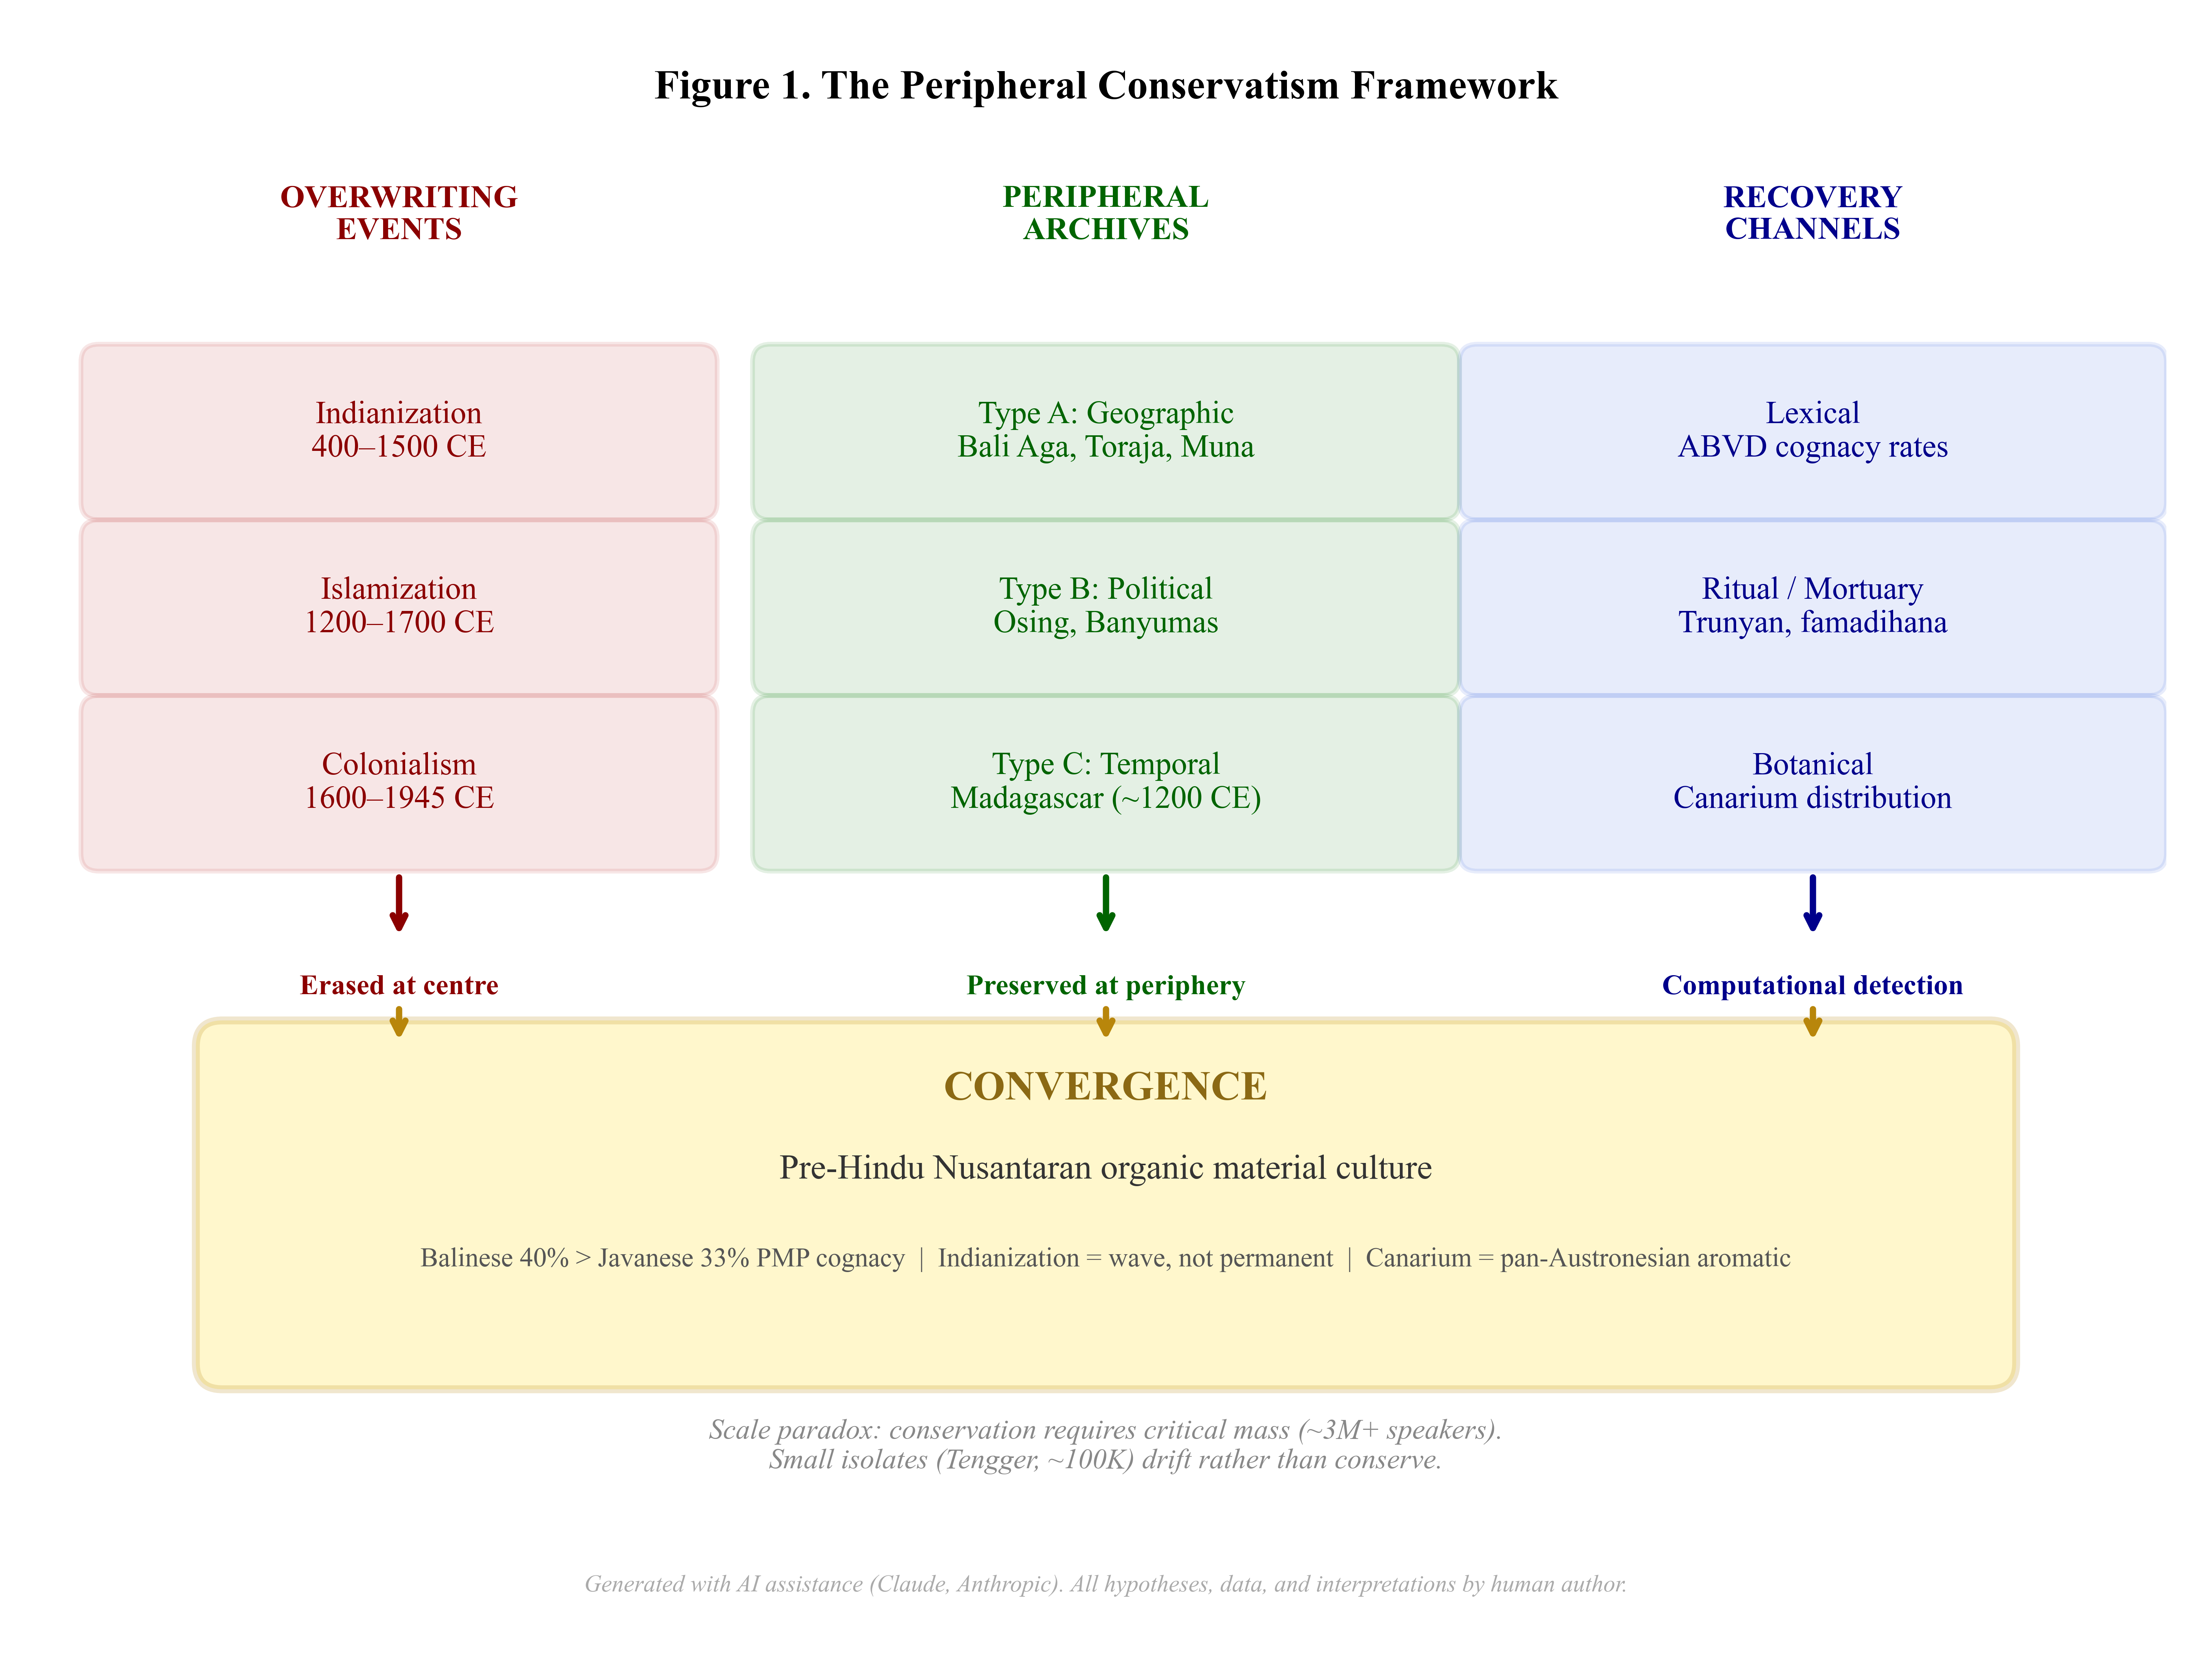
\includegraphics[width=\textwidth]{fig4_pcf_convergence.png}
\caption{The Peripheral Conservatism Framework: three overwriting events (left) erase substrates at centres, while three types of peripheral archive (centre) preserve them. Three computational recovery channels (right) detect the preserved substrates, converging on a single conclusion: a pre-Hindu organic Nusantaran material culture. Figure generated with AI assistance (Claude, Anthropic); all data and interpretations by human author.}
\label{fig:pcf}
\end{figure}

% ============================================================
% 3. LINGUISTIC CONSERVATION
% ============================================================
\section{Linguistic Conservation at the Periphery}
\label{sec:linguistic}

\subsection{Data and Method}
\label{sec:cognacy}

To test whether peripheral varieties preserve more proto-language vocabulary, we extracted forms for eight language varieties from the Austronesian Basic Vocabulary Database (ABVD) CLDF dataset:\footnote{\autocite{greenhill2008abvd}. The dataset contains 346,662 lexical forms across 2,811 language varieties for 210 basic vocabulary concepts.} Balinese (ABVD~1), Javanese (ABVD~20), Javanese of Yogyakarta (ABVD~1532), Javanese of Malang (ABVD~1534), Tengger of Ngadas (ABVD~1533), Merina Malagasy (ABVD~92), Old Javanese (ABVD~290), and Old/Middle Javanese (ABVD~1535). For each of the 210 concepts, we checked whether forms in each variety share cognate sets with PMP (ABVD~269; 201~concepts covered) or Proto-Austronesian (PAn; ABVD~280; 172~concepts).

The cognacy comparison follows the ABVD's own cognate set assignments, which are based on the work of Blust and the ABVD editorial team. A form is counted as ``PMP-cognate'' if it shares any cognate set identifier with the PMP reconstruction for the same concept. This is a conservative measure: it detects only direct lexical inheritance, not semantic or morphological parallels. Statistical comparison between language pairs uses McNemar's test, which is appropriate for paired binary data (each concept is either cognate or not in each variety).

\subsection{The Cognacy Gradient}

Results are presented in Table~\ref{tab:cognacy}. The gradient from Old Javanese (55.3\%) to modern standard Javanese (33.0\%) quantifies 22.3\% PMP cognacy erosion across approximately one thousand years of Indianization and Islamization. This is the largest gap in the dataset and represents the cumulative effect of lexical replacement by Sanskrit, Arabic, and Dutch loanwords.

\begin{table}[htbp]
\centering
\caption{PMP cognacy rates across Austronesian varieties (210 ABVD concepts). PAn = Proto-Austronesian (172 concepts covered).}
\label{tab:cognacy}
\begin{tabular}{llrrrl}
\toprule
Variety & ABVD ID & PMP \% & PAn \% & $\Delta$ vs Jav. & PCF Type \\
\midrule
Old Javanese           & 290  & 55.3 & 37.4 & +22.3 & historical baseline \\
Merina Malagasy        & 92   & 40.8 & 28.6 & +7.8  & Type C (temporal) \\
Balinese               & 1    & 40.3 & 26.7 & +7.3  & Type A (geographic) \\
\textbf{Javanese (std)} & \textbf{20} & \textbf{33.0} & \textbf{23.3} & --- & \textbf{centre} \\
Javanese (Yogyakarta)  & 1532 & 28.4 & 20.0 & $-$4.6  & sub-centre \\
Tengger (Ngadas)       & 1533 & 27.7 & 19.8 & $-$5.3  & Type A (small isolate) \\
Javanese (Malang)      & 1534 & 26.0 & 17.7 & $-$7.0  & sub-centre \\
\bottomrule
\end{tabular}
\end{table}

Merina Malagasy (40.8\%) sits between Old Javanese and modern Javanese, consistent with a \textit{c.}~1200~CE ``snapshot'' that captured the language mid-way through the erosion process. This positioning is exactly what the PCF predicts: a temporal periphery should preserve an intermediate level of proto-language cognacy, reflecting the degree of lexical replacement that had occurred by the departure date.

Balinese shows a directionally consistent greater PMP retention than standard Javanese (McNemar $\chi^2$~=~3.44, $p$~=~0.064; exact binomial test on the 36-versus-21 discordant pair: one-sided $p$~=~0.026), with 36~concepts showing peripheral advantage (Balinese retains PMP cognate while Javanese does not) versus 21~showing central advantage. While the $p$-value does not reach conventional significance at $\alpha$~=~0.05, the direction is consistent across multiple comparisons. Balinese versus Tengger is highly significant ($\chi^2$~=~13.02, $p$~=~0.0003), confirming that the two peripheral communities have diverged in opposite directions: Bali conserves, Tengger drifts.

A methodological caveat applies: ABVD wordlists for Javanese and Balinese may contain forms from high speech registers (Krama/Alus), which are disproportionately Sanskrit-derived. If Javanese forms include Krama vocabulary, PMP cognacy would be deflated for Javanese---making the Balinese advantage appear larger. However, the same confound operates in reverse for Balinese Alus. In either case, the bias is conservative: register mixing would reduce, not inflate, the true peripheral advantage. The domain-level analysis (Table~\ref{tab:domains}), which is less sensitive to individual register confounds, provides a more robust test.\footnote{An examination of the ABVD Javanese (ID~20) forms found that the wordlist predominantly contains Ngoko (low register) forms, though a small number of Krama-influenced entries may be present. The direction of any resulting bias is toward deflating Javanese PMP cognacy.}

The sub-centre varieties (Yogyakarta 28.4\%, Malang 26.0\%) show \emph{lower} PMP cognacy than the standard, suggesting that prestige court centres (Yogyakarta as the historical seat of Mataram; Malang as a post-Singhasari centre) undergo more intensive lexical replacement than the standardized reference variety.

\begin{figure}[htbp]
\centering
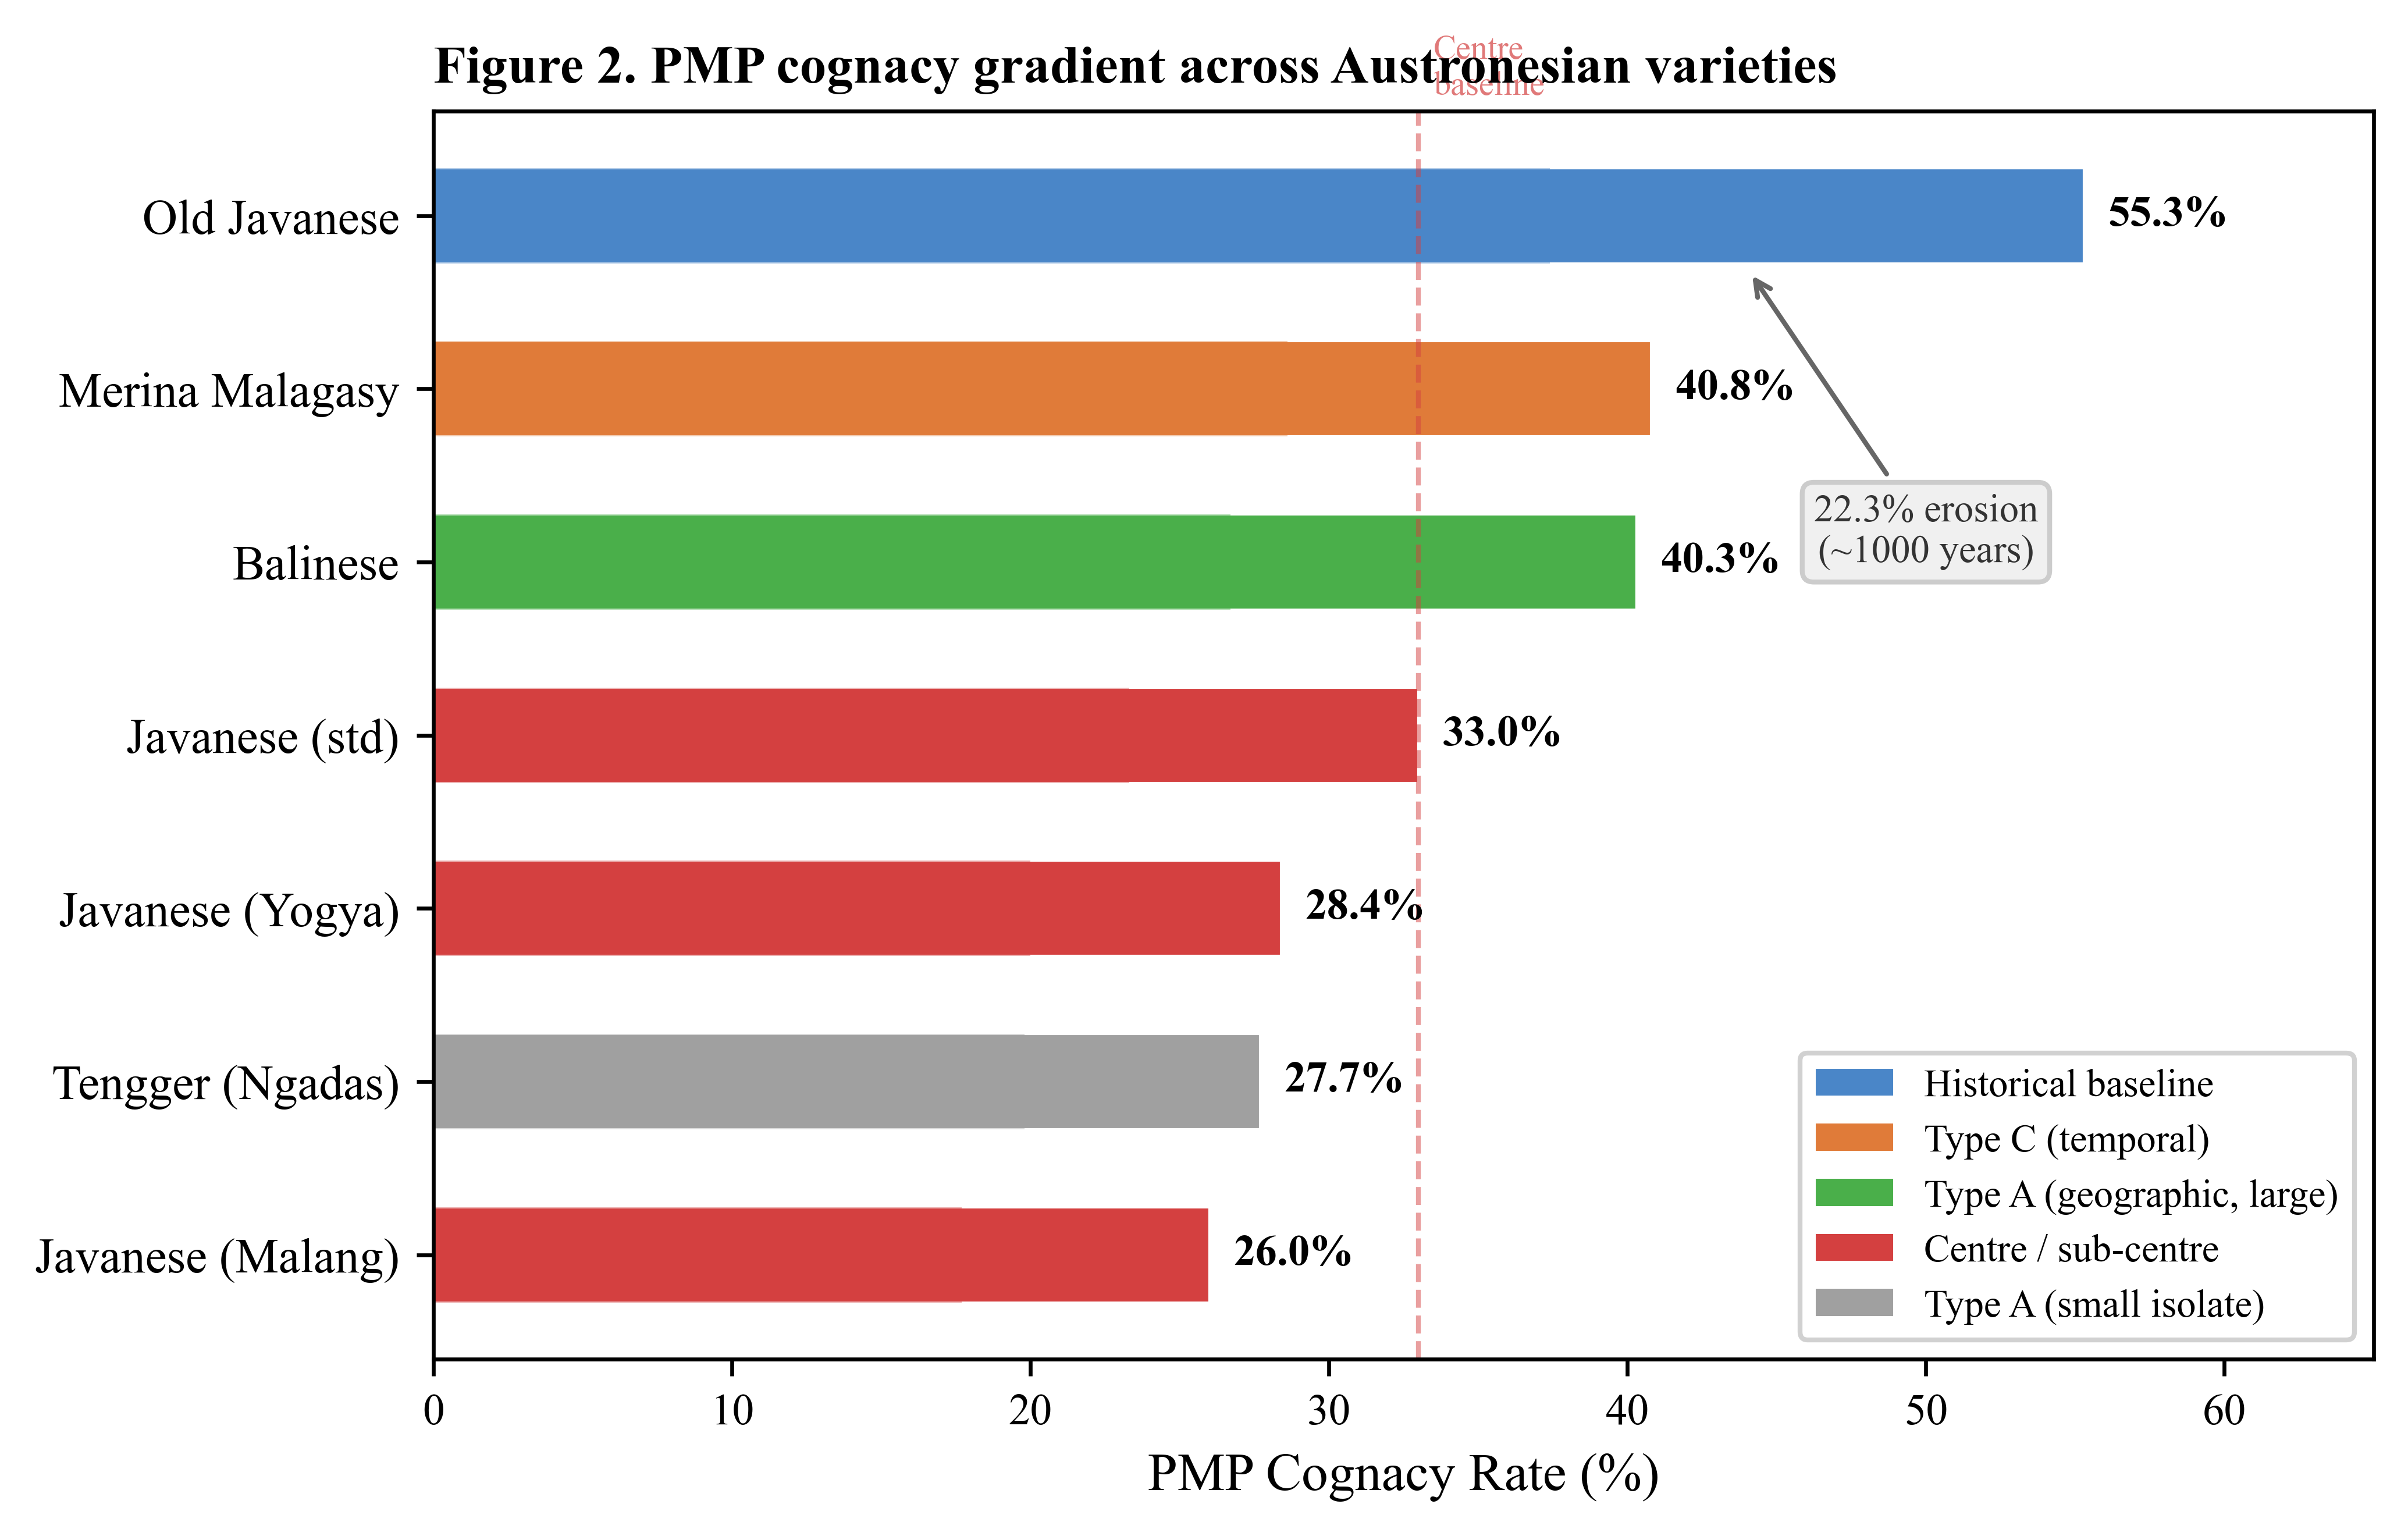
\includegraphics[width=0.95\textwidth]{fig1_cognacy_gradient.png}
\caption{PMP cognacy gradient across Austronesian varieties, colour-coded by PCF type. The 22.3\% gap between Old Javanese and modern Javanese quantifies approximately one thousand years of lexical erosion. Peripheral varieties (Balinese, Malagasy) retain more proto-language vocabulary than the centre; the small isolate (Tengger) drifts below the centre. Dashed line marks the Javanese standard baseline.}
\label{fig:cognacy}
\end{figure}

\subsection{Semantic Domain Concentration}

The peripheral advantage is not uniform across vocabulary domains. Table~\ref{tab:domains} shows PMP cognacy rates by semantic domain for four key varieties.

\begin{table}[htbp]
\centering
\caption{PMP cognacy rates (\%) by semantic domain.}
\label{tab:domains}
\begin{tabular}{lrrrr}
\toprule
Domain & Balinese & Javanese & Tengger & Malagasy \\
\midrule
NATURE  & 72.7 & 45.5 & 36.4 & 54.5 \\
NUMBER  & 50.0 & 50.0 & 100.0 & 50.0 \\
KINSHIP & 25.0 & 12.5 & 12.5 & 50.0 \\
BODY    & 30.0 & 30.0 & 33.3 & 50.0 \\
ACTION  & 20.8 & 29.2 & 25.0 & 45.8 \\
OTHER   & 40.2 & 32.0 & 23.1 & 34.4 \\
\bottomrule
\end{tabular}
\end{table}

Nature-domain terms---earth, stone, water, fire, tree, leaf, and similar---show the largest peripheral advantage (+27.2\% for Balinese over Javanese). This is consistent with the hypothesis that \emph{landscape vocabulary}, describing the physical environment, is most resistant to prestige-driven replacement, precisely because the landscape itself does not change with cultural overlay. A new court may impose Sanskrit titles and ritual terminology, but it cannot rename the rain.

Among the 36~concepts where Balinese retains PMP cognacy while Javanese does not, we find: \emph{earth/soil}, \emph{fire}, \emph{leaf}, \emph{flower}, \emph{stone}, \emph{rain}, \emph{lake}, \emph{dust}, \emph{cold}---overwhelmingly landscape and natural-world terms. The 21~concepts where Javanese retains PMP but Balinese does not are more varied: \emph{dog}, \emph{bird}, \emph{mosquito}, \emph{tongue}, \emph{nose}---terms for which Balinese has innovated, perhaps under the influence of Balinese-specific speech levels (\emph{Alus}/\emph{Kasar}).

\begin{figure}[htbp]
\centering
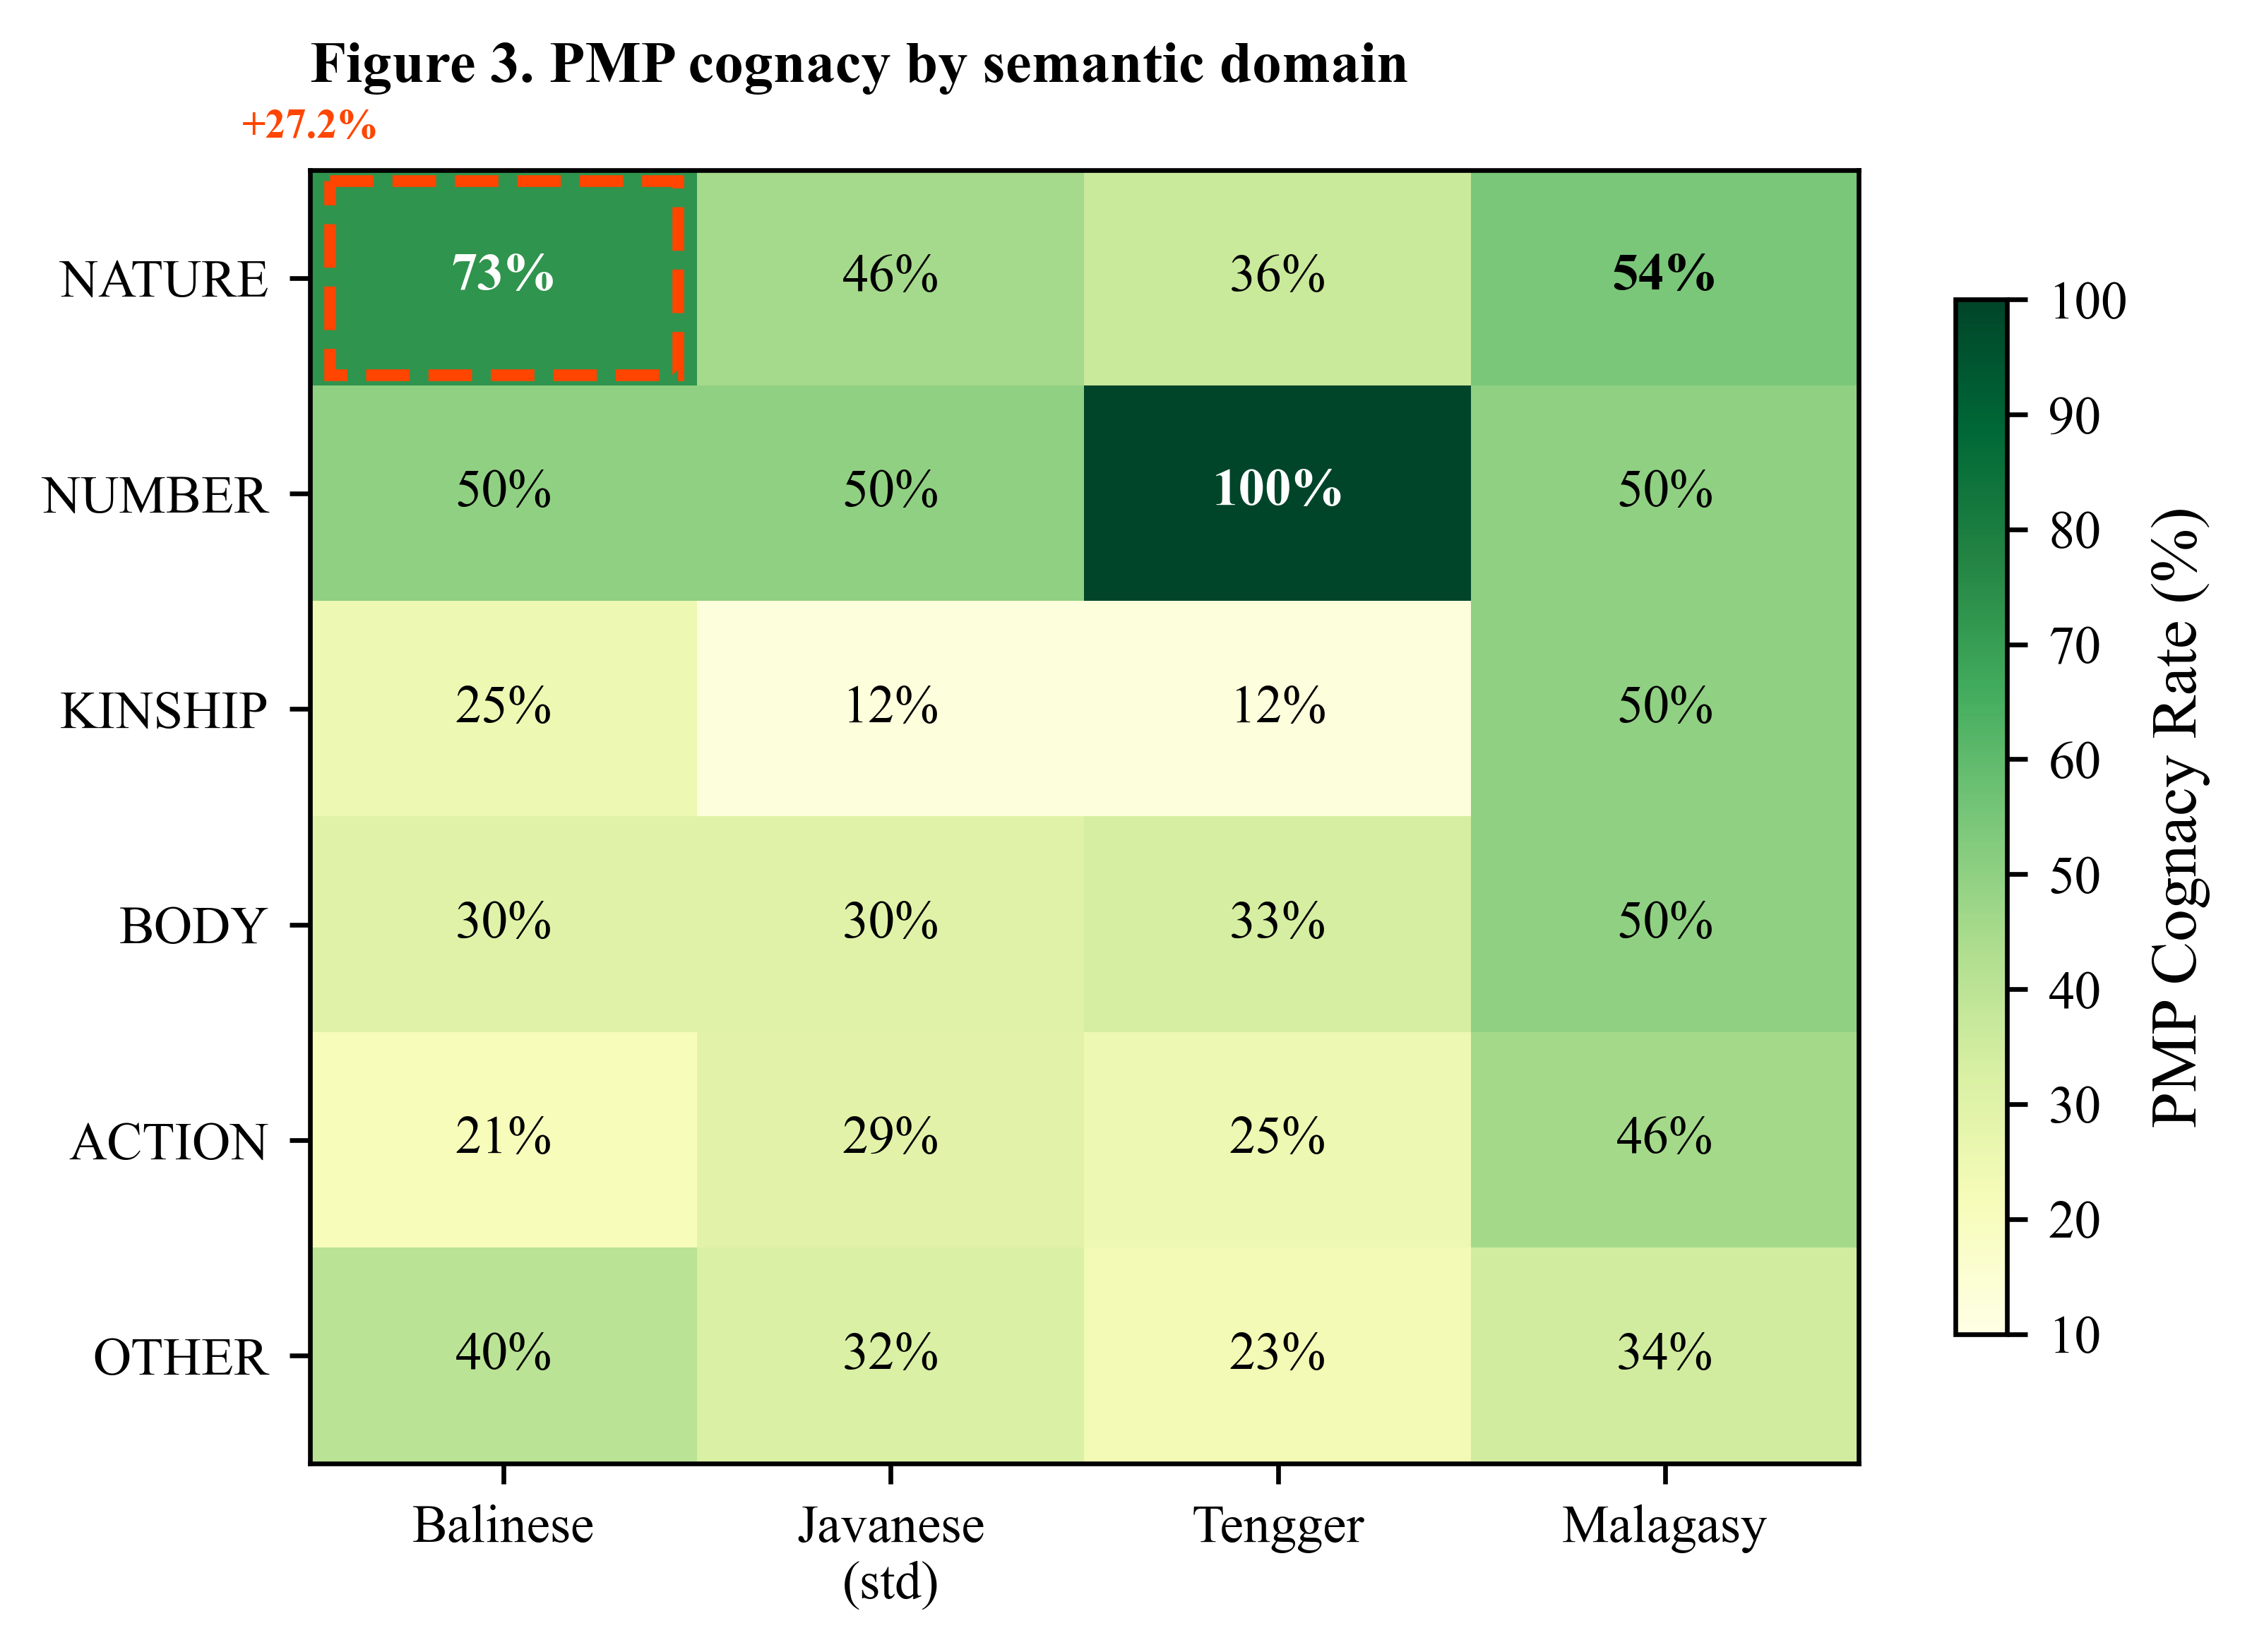
\includegraphics[width=0.75\textwidth]{fig6_domain_heatmap.png}
\caption{PMP cognacy rates by semantic domain across four key varieties. The dashed box highlights the largest peripheral advantage: Balinese NATURE domain (73\%) versus Javanese (46\%). Tengger's 100\% numeral retention (dark cell) shows domain-specific conservation even in a drifting system.}
\label{fig:heatmap}
\end{figure}

Two anomalies deserve note. First, Tengger's 100\% numeral retention: all basic numerals in this small isolate retain PMP cognacy, even as general vocabulary drifts. This accords with the well-known stability of numeral systems cross-linguistically and suggests that functional domains (counting, trading) resist drift even in small populations. Second, Malagasy shows the highest kinship cognacy (50\%)---twice the Javanese rate---suggesting that kinship terminology was replaced in Java by Indic kin terms (\emph{putra}, \emph{putri}, \emph{dewa}) while Madagascar preserved the Austronesian system.

\subsection{The Indianization Wave}
\label{sec:wave}

The cognacy gradient represents the endpoint of a process that proves non-monotonic when examined diachronically. Analysis of Sanskrit/Indic vocabulary ratios across 268 dated DHARMA inscriptions reveals a wave pattern rather than a monotonic increase:\footnote{See \autocite{amien2026c} for full methodology. The relevant experiment (E033) classified each ritual keyword-token in 268 inscriptions as Indic or non-Indic using etymological dictionaries, then computed the ratio per inscription over time.}

\begin{itemize}
\item Peak Indianization: century~9 (Medang/Mataram period), Indic ratio = 0.807
\item Trough: century~13 (Singhasari/early Majapahit), Indic ratio = 0.569
\item Temporal trend: Spearman $\rho$ = $-$0.211, $p$ = 0.030 (significant decline)
\item Language shift: Sanskrit inscriptions dominate centuries~6--8 (43--100\%), then virtually disappear; centuries~9--14 are 83--100\% Old Javanese
\item Pre-Indic term diversity: 1~unique term (C8--C9: only \emph{hya\.m}) expanding to 5+~terms (C10--C11: \emph{hya\.m}, \emph{ma\.nghuri}, \emph{gunung}, \emph{panumbas}, \emph{hyang})
\end{itemize}

Indianization was a \textbf{wave} that crested in the ninth century and receded, with pre-Indic vocabulary diversifying as the wave retreated. The indigenous 210-day calendar (\emph{wuku}) appears only in thirteenth- and fourteenth-century inscriptions, suggesting a late-stage substrate reassertion. The conventional periodization---which treats the ``end'' of Hindu-Buddhism in Java (fifteenth century, fall of Majapahit) as a rupture---misreads what was in fact a gradual substrate reassertion that had been underway for at least four centuries.

\begin{figure}[htbp]
\centering
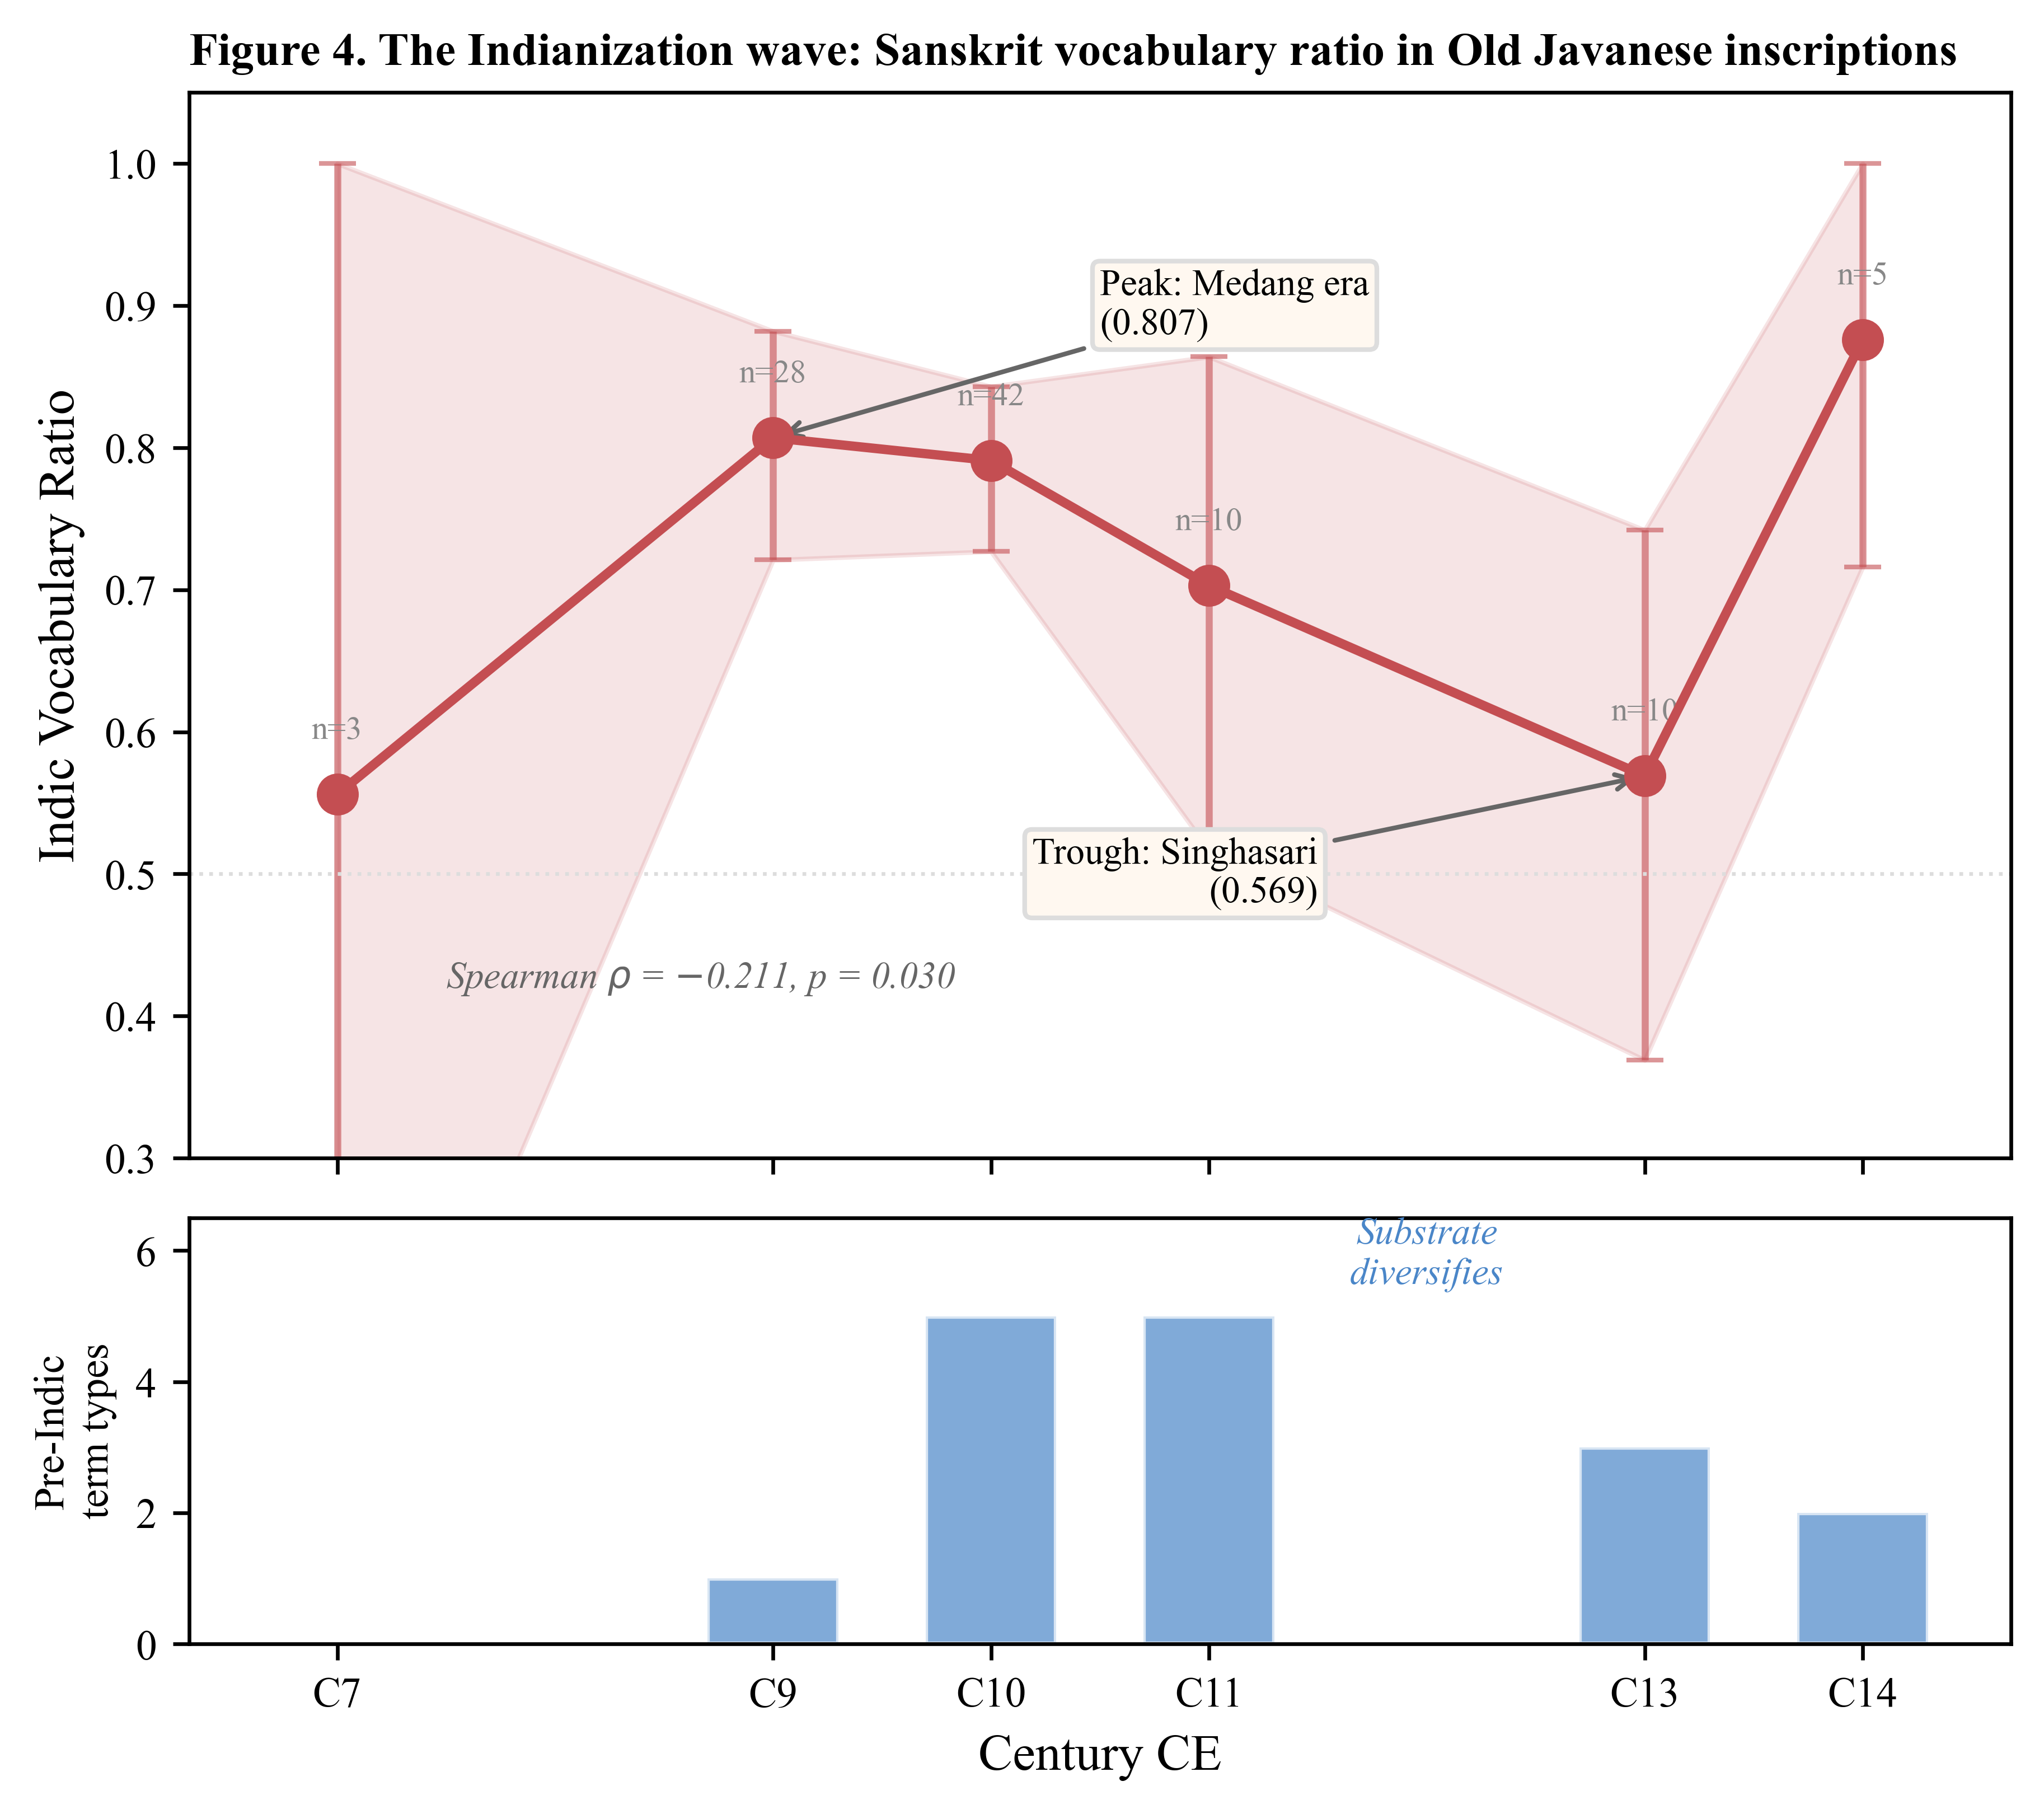
\includegraphics[width=0.9\textwidth]{fig2_indianization_wave.png}
\caption{The Indianization wave. Top panel: Indic vocabulary ratio in dated Old Javanese inscriptions, showing peak at century~9 (Medang era, 0.807) and trough at century~13 (Singhasari, 0.569). Shaded area: 95\% confidence interval. Bottom panel: diversity of pre-Indic term types per century, showing substrate vocabulary diversifying as the Indic wave recedes. Data from 268 DHARMA inscriptions (E033).}
\label{fig:wave}
\end{figure}

This finding has direct implications for the PCF: it means that the Indianization ``overwriting'' was not complete even at the centre. The substrate was always present, merely submerged beneath the prestige layer, and it resurfaced as the prestige wave receded. What peripheries preserve openly, centres preserve covertly---detectable only through computational corpus analysis.

\subsection{Phonological Confirmation}

Independent confirmation comes from Hanacaraka script analysis.\footnote{\autocite{amien2026d}, experiment E036. The analysis compares the phonological inventory encoded in the Hanacaraka script (used for Javanese, Balinese, and Sundanese) with the inventories of Sanskrit and Proto-Austronesian.} The reduction from 33~Sanskrit consonants to 20~Hanacaraka characters reveals systematic loss of precisely those phonological categories that Proto-Austronesian lacks: aspiration (8~consonants lost), retroflexes (5), and sibilant distinctions (2). The resulting 20-consonant inventory aligns with Proto-Austronesian ($\sim$17~consonants), not with Sanskrit (33).

The implication is that the script was not passively adopted but actively fitted to a pre-existing phonological system---the shape of the glove reveals the shape of the hand. Two paradoxes within this pattern merit further investigation: the retention of \emph{tha} and \emph{dha} (which have no PAn source, suggesting possible substrate retention from a non-Austronesian language), and the phonemic status of the glottal stop /?/ in Javanese, which is productive but unrepresented in the Hanacaraka script---a pre-script feature that the writing system never captured.

\subsection{Machine Learning Substrate Detection}

An exploratory, supplementary line of evidence comes from computational substrate detection using machine learning.\footnote{\autocite{amien2026d}. The model uses XGBoost trained on phonological features (form length, consonant cluster frequency, glottal stops, prefix patterns, semantic domain) to distinguish inherited Austronesian vocabulary from substrate candidates. We present this as exploratory evidence rather than a primary pillar of the argument; the PCF does not depend on the ML results.} An XGBoost classifier trained on phonological features of six Western Malayo-Polynesian languages achieves AUC~=~0.760 (cross-validated) with leave-one-language-out (LOLO) validation showing 5 of 6~languages at AUC~$\geq$~0.65.

The most informative features for substrate detection are: language-specific cognacy coverage, form length (substrates are longer), semantic domain (action verbs dominate substrates at 46\% of the top~50 candidates), consonant cluster frequency, and the presence of glottal stops. This phonological ``fingerprint'' of substrate vocabulary has been validated against two potential confounds: orthographic approximation (IPA conversion changes AUC by only +0.002)\footnote{Experiment E041.} and length metric choice (syllable-based versus character-based measures produce equivalent results; removing length features entirely yields AUC~=~0.769).\footnote{Experiment E042.}

The dominance of action verbs among substrate candidates is diagnostically important: everyday activities (cutting, carrying, planting, cooking) are described in pre-Sanskrit vocabulary, while abstract and cosmological terms are Indic. The substrate vocabulary describes the same organic, material world that is independently attested in the inscription record (see~\S\ref{sec:organic}) and independently destroyed by volcanic taphonomy.

% ============================================================
% 4. MORTUARY AND BOTANICAL CONSERVATION
% ============================================================
\section{Mortuary and Botanical Conservation}
\label{sec:mortuary}

\subsection{The Trunyan Case}

The Bali Aga of Trunyan practise \emph{mepasah}: exposed above-ground burial, the body placed under the Taru Menyan tree, decomposition by natural processes, bones later collected at the site periphery.\footnote{\autocite{danandjaja1980kebudayaan}; see also \autocite{astiti2005trunyan}.} The village is situated on the western shore of Lake Batur, inside the caldera of the still-active volcano, accessible historically only by boat. This geographic isolation has preserved a burial practice that differs fundamentally from both Hindu-Balinese cremation and Islamic inhumation.

Key structural elements of the Trunyan mortuary system include: (1)~no inhumation---bodies are not buried underground; (2)~no cremation---bodies are not burned; (3)~botanical neutralization of decomposition odour through proximity to the aromatic Taru Menyan tree; (4)~tripartite cemetery classification by death-type (natural death, accidental death, and infant/child death each have separate burial areas); (5)~volcanic context---the site is adjacent to active Mt~Batur, and the community maintains awareness of volcanic hazard; and (6)~the explicit belief that improper burial practices can cause volcanic eruption.

Element~(6) is remarkable: the community links mortuary practice to volcanic activity directly, not metaphorically---Mt~Batur is active and visible from the cemetery, with historical eruptions in living memory. Whether causation runs from volcano to ritual (volcanic hazard motivates careful mortuary practice) or from ritual to volcano (proper burial maintains cosmic balance) is undeterminable from ethnography alone, but the association is robust and distinguishes Trunyan from non-volcanic peripheral burial sites.

The antiquity of the Trunyan community is attested epigraphically: a copper plate inscription dated 833~\v{S}aka (\textit{c.}~911~CE) was found at the Trunyan temple, and a bronze tablet of the same date exists at Pura Tegeh Koripan on nearby Mt~Penulisan.\footnote{Balinese copper plate inscriptions; see the DHARMA digital corpus at \url{https://github.com/erc-dharma} for TEI-XML editions.} The temple architecture predates the inscription, placing the settlement at least in the ninth century and possibly considerably earlier.

\subsection{Cross-Regional Mortuary Parallels}

Structural comparison across Austronesian communities reveals a shared mortuary pattern (Table~\ref{tab:mortuary}). Malagasy \emph{famadihana} (bone-turning ritual, performed on a cycle of approximately seven years) and Toraja \emph{ma'nene} (annual bone-cleaning ceremony) are structurally homologous: both involve secondary treatment of skeletal remains with strong community participation requirements and textile wrapping of bones. The Toraja \emph{tau-tau}---carved wooden effigies placed in cliff-face galleries---represents an additional layer of above-ground mortuary display that finds no direct parallel in Madagascar but echoes the Trunyan practice of maintaining visible bone collections at the cemetery periphery.

\begin{table}[htbp]
\centering
\caption{Cross-regional mortuary structural parallels across Austronesian peripheries.}
\label{tab:mortuary}
\begin{tabular}{p{3.5cm}ccc}
\toprule
Element & Trunyan & Toraja & Malagasy \\
\midrule
Exposed/above-ground phase  & \checkmark & \checkmark & \checkmark \\
Secondary bone treatment    & \checkmark & \checkmark & \checkmark \\
Aromatic botanical element  & \checkmark & ?          & \checkmark \\
Community participation     & \checkmark & \checkmark & \checkmark \\
Textile wrapping of bones   & partial    & \checkmark & \checkmark \\
Sacred tree association     & \checkmark & \checkmark & \checkmark \\
\bottomrule
\end{tabular}
\end{table}

This structural homology across communities separated by 6,000~km of ocean (Indonesia to Madagascar) and 2,000~km of land (Bali to Sulawesi) is more parsimoniously explained by shared Austronesian ancestral practice than by convergent evolution. To be sure, exposed burial and secondary bone treatment occur independently in other cultural traditions---Tibetan sky burial, Zoroastrian \emph{dakhma}, and various Pacific island mortuary rites all involve above-ground body disposition. However, the convergent-evolution objection must account not for any single element but for the \emph{specific combination} of six elements (Table~\ref{tab:mortuary}): exposed body phase, secondary bone treatment, aromatic botanical element, community participation requirement, textile wrapping, and sacred tree association. This combination is absent from the geographically \emph{intervening} Hindu-Balinese and Islamic Javanese traditions, which favour cremation and rapid inhumation respectively. Convergent evolution would predict the shared pattern to appear also in these intervening populations, which it does not. The peripheral pattern is precisely what the PCF predicts would survive in communities that escaped or resisted overwriting events.

\subsection{The Botanical Substitution Chain---Revised}
\label{sec:botanical}

A critical finding of this study concerns the aromatic tree ubiquitous at Javanese Muslim cemeteries: \emph{Plumeria}~spp. (kamboja/frangipani). Informants consistently explain its presence as odour-neutralization---functionally identical to the Trunyan explanation for Taru Menyan. The assumption, common in ethnographic literature, is that kamboja represents a continuous tradition linking modern burial practice to pre-Hindu custom.

However, \textbf{\emph{Plumeria} is a New World species}, native to Mexico, Central America, and the Caribbean. The genus was named by Tournefort in 1700 in honour of Charles Plumier, who explored the tropical Americas. It was introduced to the Philippines by Spanish colonists in the 1560s and subsequently spread to Indonesia via colonial botanical exchange.\footnote{On the introduction of New World species to Island Southeast Asia via the Manila-Acapulco galleon trade and Portuguese Estado da \'{I}ndia, see the broader literature on the Columbian Exchange in Southeast Asia. Plumeria reached Indonesia no earlier than the late sixteenth century.} \emph{Plumeria} therefore \emph{cannot} be a pre-Hindu aromatic burial tree. Its presence at Javanese cemeteries is a post-1560 adoption, not a survival.

This requires a revision of the botanical substitution model from three layers to four:

\textbf{Layer~1---Pre-Hindu ($\sim$pre-400~CE):} Exposed burial with native aromatic tree. Taru Menyan at Trunyan survives as the sole documented example in Java/Bali. The broader Austronesian candidate is \textit{Canarium}~spp., a resin-producing tree of the Burseraceae family used as ceremonial incense across the Austronesian range. \textit{C.~madagascariense} (ramy or haramy) serves as ceremonial incense in Madagascar;\footnote{Beaujard documents Canarium resin use in Malagasy ceremonial contexts; the tree is cultivated in sacred forests near tombs.} \textit{C.~strictum} (dammar/sambrani) fills the same function in Indonesian religious ceremonies; \textit{C.~indicum} is documented as ``among the oldest and most important tree crops'' in Melanesia,\footnote{\autocite{yen1995canarium}. Canarium is used for resin (canoe caulking, incense), edible nuts, and ceremonial face paint across Island Melanesia.} where it has been cultivated since early Austronesian settlement. The pan-Austronesian distribution of \textit{Canarium} in ceremonial contexts---spanning from Melanesia through Indonesia to Madagascar---makes it the strongest candidate for the pre-Hindu aromatic burial tree.

An alternative candidate deserves consideration: \textit{Styrax benzoin} (kemenyan/menyan), the resin-producing tree native to Sumatra and a major pre-modern trade commodity. The very name ``Tru Menyan'' at Trunyan likely derives from \emph{menyan} (benzoin), making \textit{Styrax} the most locally attested candidate for the Bali-Java context. The two candidates are not mutually exclusive: the pre-Hindu aromatic burial tree may have varied regionally, with \textit{Styrax} predominating in the western Nusantaran zone (Sumatra, Java, Bali) and \textit{Canarium} spanning the broader Austronesian world from Melanesia to Madagascar. Both are indigenous, both produce aromatic resin, and both have documented ceremonial functions. The critical point for the PCF is not which specific species served the burial function, but that an indigenous aromatic tree tradition existed \emph{before} \textit{Plumeria} replaced it---and that this tradition is recoverable through peripheral and temporal archives.

\textbf{Layer~2---Indianization ($\sim$400--1200~CE):} Inhumation becomes dominant in court-influenced areas. The aromatic botanical element is retained but its function shifts from ``decomposition neutralizer'' (exposed burial) to ``grave marker/purifier'' (inhumation). Cendana (sandalwood, \textit{Santalum album}) appears in this layer---present in 11 of 268~DHARMA inscriptions, always in ritual context (100\% co-occurrence with ritual keywords).\footnote{Experiment E035. Cendana's consistent ritual association distinguishes it from economic plants like rice or cotton.}

\textbf{Layer~3---Islamization ($\sim$1200--1560~CE):} Inhumation is reinforced by Islamic burial requirements. The native aromatic tree tradition continues, but which species served this role before \emph{Plumeria} arrived remains unattested in Java proper. The gap is itself evidence: the replacement was complete enough to erase the predecessor's identity.

\textbf{Layer~4---Portuguese contact ($\sim$1560s onward):} \emph{Plumeria} introduced from the Americas, adopted at cemeteries because of its similar aromatic properties, rapid growth, and tolerance of poor soil. It replaces whatever native species---\emph{Canarium}? an endemic aromatic?---had served the burial function.

\begin{figure}[htbp]
\centering
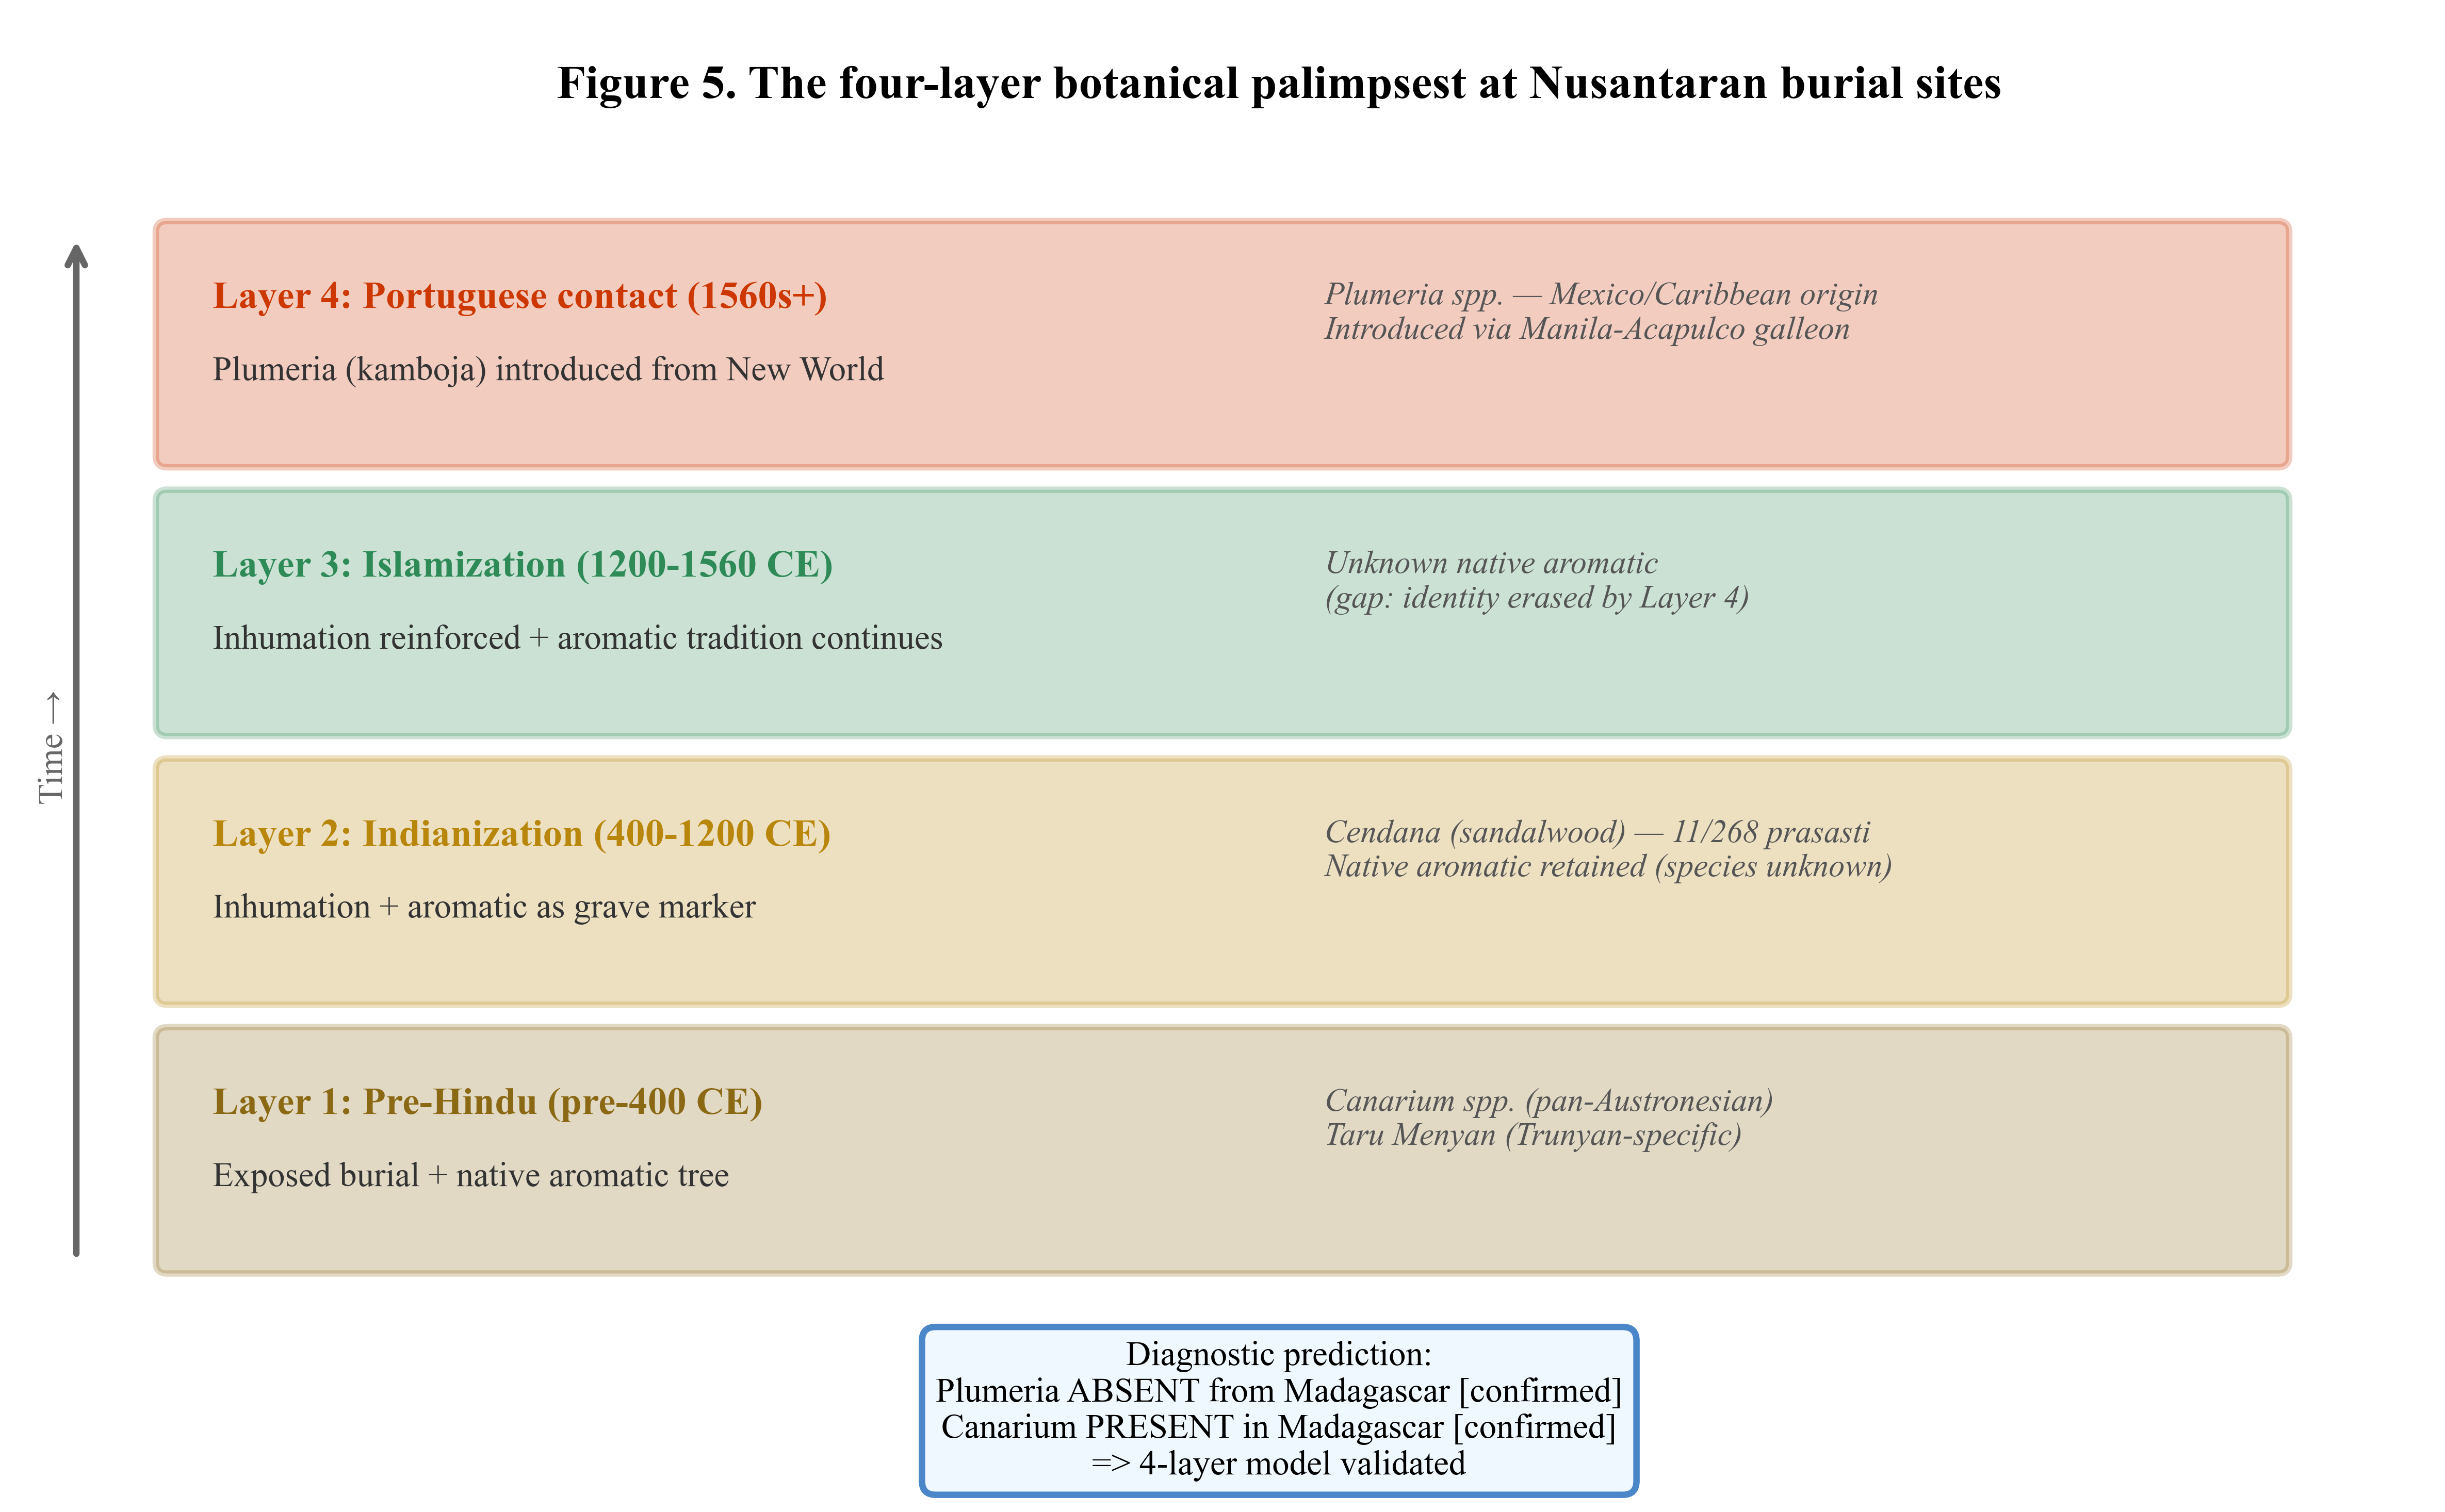
\includegraphics[width=\textwidth]{fig3_botanical_layers.png}
\caption{The four-layer botanical palimpsest at Nusantaran burial sites. The pre-Hindu aromatic tree (\textit{Canarium}~spp.) was successively overlaid by Indianization, Islamization, and Portuguese-era introduction of New World \textit{Plumeria}. The diagnostic prediction---\textit{Plumeria} absent from Madagascar, \textit{Canarium} present---is consistent with the model.}
\label{fig:botanical}
\end{figure}

The diagnostic prediction of this four-layer model is consistent with the Malagasy evidence: \emph{Plumeria} does \emph{not} appear in Malagasy burial contexts (the migration predates introduction by over 300~years), but \emph{Canarium} \emph{is} present as ceremonial aromatic in Madagascar. The absence of \emph{Plumeria} and presence of \emph{Canarium} in Madagascar is exactly what the model predicts---and what any model positing \emph{Plumeria} as a pre-Hindu aromatic tree cannot explain.

\subsection{Sacred Forests and Botanical Taboos}

Additional structural homology appears in vegetation treatment around burial sites. In Madagascar, sacred forests (\emph{ala masina}) around tombs are strictly protected: cutting trees or burning dead wood is forbidden (\emph{fady}), and ecological surveys have documented 35~woody species unique to \emph{fady}-protected tomb forests that do not occur in adjacent non-protected areas. Ancestors are believed to reside in sacred trees (\emph{hazofaly}). Among the Mikea people, dead infants are placed in baobab branches rather than buried---a structural parallel to Trunyan exposed burial that places the body \emph{in} the tree rather than \emph{under} it.

In Java and Bali, sacred groves around temples and cemeteries serve the identical function, with botanical taboos (\emph{larangan} or \emph{pamali}) protecting specific species. Ancestors are associated with the waringin (banyan, \textit{Ficus benjamina}), which appears in 114 of 268~DHARMA inscriptions (42.5\%) with 93\% ritual context co-occurrence---making it the most pervasive sacred tree in the Javanese epigraphic record.\footnote{Experiment E035.} The parallel between Malagasy \emph{fady} and Javanese \emph{pamali} is not merely structural (protected forest around burial site) but functional (botanical taboo preserves specific species through supernatural sanction) and possibly etymological---both terms denote supernatural prohibition without clear Indic source.

\subsection{Mortuary Plants versus the Epigraphic Record}

Screening of 268 DHARMA inscriptions for botanical terms reveals that 249 (92.9\%) contain plant references.\footnote{Experiment E035. Top plants: \emph{padi} (81\%), \emph{waringin} (43\%), \emph{tebu} (16\%), \emph{sirih} (16\%), \emph{padma} (11\%), \emph{cendana} (4\%), \emph{kapur barus/camphor} (3\%).} However, the mortuary-specific plants---\emph{menyan} (benzoin incense) and \emph{kamboja}---are \textbf{completely absent} from the epigraphic record, despite \emph{menyan} being the namesake of the most archaic surviving burial site (Taru Menyan, Trunyan) and benzoin being one of the most important trade commodities of Sumatra.

This absence is diagnostic. It reveals two distinct registers of botanical knowledge: a \emph{state/administrative register} recorded in stone inscriptions (land grants, tax bases, boundary markers: rice, sugarcane, cotton, banyan) and a \emph{mortuary/oral register} transmitted outside the epigraphic system entirely. The \emph{prasasti} record the Indianized administrative surface; mortuary botanical practice lived underneath, transmitted orally, and therefore invisible to epigraphy-based historiography. The distinction parallels the broader PCF argument: what survives at the centre (inscriptions) reflects the prestige overlay; what survives at the periphery (living practice) reflects the substrate.

% ============================================================
% 5. THE ORGANIC CIVILIZATION
% ============================================================
\section{The Organic Material World and Genre Taphonomy}
\label{sec:organic}

\subsection{Material Culture in the Inscriptions}

Systematic screening of 268 DHARMA inscriptions for references to organic and lithic building materials yields a striking asymmetry:\footnote{Experiment E040. Organic keywords: \emph{daun} (leaf/thatch), \emph{atap} (roof/thatch), \emph{kayu} (wood), \emph{ijuk} (palm fibre), \emph{bambu} (bamboo), \emph{rotan} (rattan), \emph{jati} (teak). Lithic keywords: \emph{batu} (stone), \emph{sela} (rock), \emph{watu} (stone), \emph{candi} (stone temple), \emph{prasada} (shrine).}

\begin{itemize}
\item Organic materials: 170/268 (63.4\%) of inscriptions; 377~total mentions
\item Lithic materials: 73/268 (27.2\%); 89~total mentions
\item Organic-only inscriptions: 103
\item Lithic-only inscriptions: 6
\item Binomial test for organic versus lithic in paired inscriptions: $p$ < 0.0001
\end{itemize}

The top organic keywords by frequency are: \emph{daun} (48\%), \emph{atap} (32\%), \emph{kayu} (26\%), \emph{ijuk} (18\%), and \emph{bambu} (10\%). The material world recorded in these inscriptions is overwhelmingly organic: wood, bamboo, palm fibre, thatch, rattan. Lithic materials appear primarily in the form of \emph{batu} (stone, 13\% of inscriptions)---the generic term---rather than as finished architectural elements.

\begin{figure}[htbp]
\centering
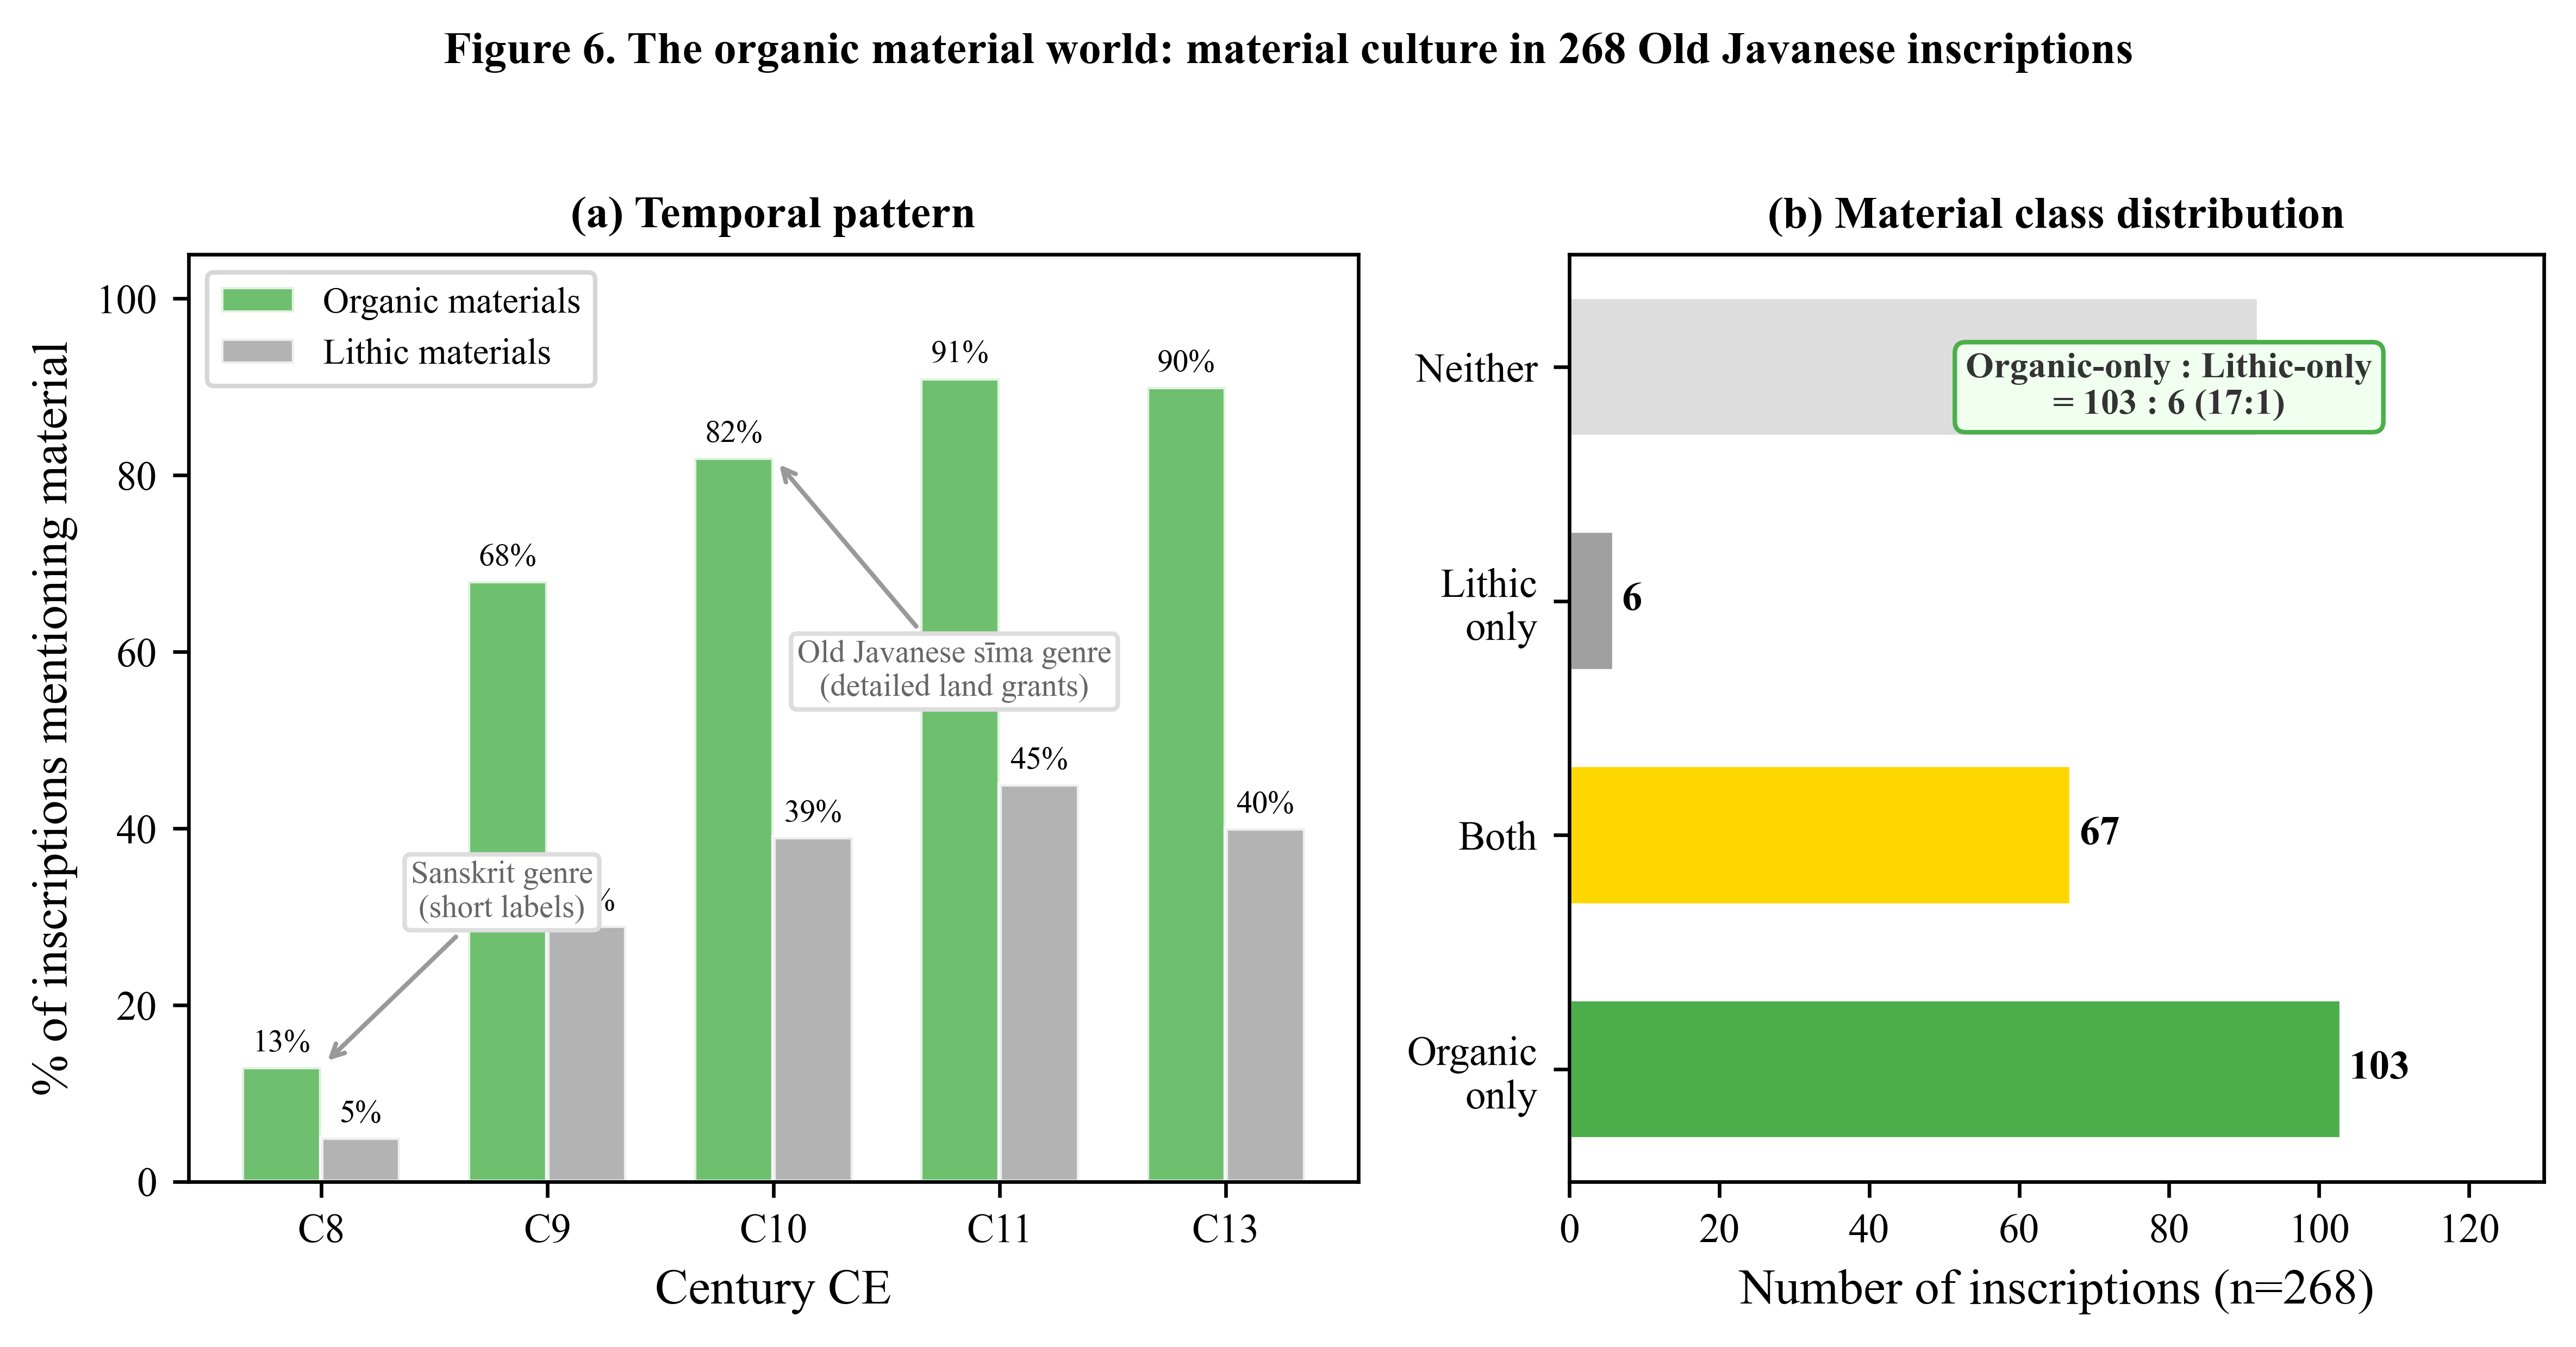
\includegraphics[width=\textwidth]{fig5_organic_civilization.png}
\caption{Material culture in 268 Old Javanese inscriptions (DHARMA corpus). (a)~Temporal pattern: organic material mentions rise from 13\% in century~8 (Sanskrit genre) to 82--91\% in centuries~9--11 (Old Javanese \emph{s\={\i}ma} genre), reflecting genre taphonomy rather than material-cultural change. (b)~Overall distribution: 103~inscriptions mention organic materials only, versus 6~lithic-only (ratio 17:1). Data from E040.}
\label{fig:organic}
\end{figure}

There is an irony in this finding that deserves emphasis: the \emph{prasasti} are themselves stone objects. They are the most durable medium their society possessed. Yet even these stone monuments record a material world of leaf, wood, and fibre. The inscriptions are not describing what we would find if we excavated---they are describing what we have lost.

\subsection{The Craft Economy}

An additional scan for craft occupation keywords reveals the workforce behind this organic economy.\footnote{Experiment E040b.} Organic craftspeople---\emph{undahagi} (carpenter), weavers, thatchers---appear in 29 inscriptions (10.8\%) with 55~total mentions. Lithic craftspeople---\emph{pandai batu} (stone mason), sculptors---appear in a comparable 31 inscriptions (11.6\%) but with only 32~total mentions. The organic-to-lithic craft mention ratio is 1.7:1, less dramatic than the 4.2:1 material ratio because the workforce was integrated: carpenters and stone masons co-occur in 11 of 16~inscriptions that mention both. Even stone temples required organic craftspeople---for scaffolding, roofing, temporary structures, and ritual preparations.

\subsection{Genre Taphonomy}

The screening also reveals an unexpected temporal pattern: century-8 inscriptions mention organic materials at only 13\%, while century-9--11 inscriptions mention them at 68--91\%. This dramatic increase does not reflect a change in material culture---it reflects a change in the \emph{genre of inscription}.

Century-8 inscriptions are predominantly short Sanskrit-language boundary markers and dedicatory labels---the Borobudur gallery labels alone account for 48 entries of median length 1,364~characters. These texts are formatted as brief Sanskrit verses that name a deity, a donor, or a location. They do not describe economic activity. Century-9 and later inscriptions are overwhelmingly Old Javanese-language \emph{sima} (land grant) documents---detailed administrative texts averaging 5,464~characters that enumerate taxable occupations, building materials, agricultural products, and craft activities.

The statistical relationship is clear: \emph{sima}-genre inscriptions mention organic materials at 84.7\%, versus 33.6\% for non-\emph{sima} inscriptions (odds ratio~=~10.96, $p$~<~0.000001). The genre---not the material culture---determines what is recorded. To be sure, the emergence of the \emph{s\={\i}ma} genre itself reflects real political transformation: the Mataram state's expansion into rural economic administration required a documentary format that enumerated taxable resources. But the material world that \emph{s\={\i}ma} inscriptions describe---organic craftwork, bamboo construction, palm-fibre processing---was pre-existing, not created by the genre change. The \emph{s\={\i}ma} format created a wider aperture onto an economy that was already there. Sanskrit-format inscriptions are a narrow aperture that admits only cosmological and dedicatory content. Old Javanese \emph{sima} inscriptions are a wide aperture that admits the full material world. The organic economy was always there; century-8 simply was not writing about it.

This constitutes a \textbf{genre taphonomy}: the form of the textual record acts as a filter on what cultural information reaches the present. It is a taphonomic process operating on information rather than matter, with the same result---systematic loss of specific categories from the recoverable record. The implication for historiography is significant: the apparent ``emergence'' of complex Javanese civilization in the ninth century is partly an artefact of genre change from Sanskrit dedicatory to Old Javanese administrative inscription, not evidence that complex social organization appeared \emph{de novo}.

\subsection{The Convergence}

The organic material-culture finding bridges two otherwise separate lines of argument:

\begin{enumerate}
\item Volcanic burial physically destroys organic archaeological evidence at 2.4--6.2~mm/year.\footnote{\autocite{amien2026a}.} A bamboo structure buried under 4~mm/year of volcanic sediment leaves no recoverable trace after several centuries.

\item Linguistic substrate detection reveals non-Sanskrit vocabulary overwhelmingly concentrated in action verbs (46\% of the top~50 machine-learning-detected substrates):\footnote{\autocite{amien2026d}, experiment E027.} cutting, carrying, planting, cooking---the everyday activities of an organic-material economy.

\item The inscription record itself indicates that the described material culture was predominantly organic (63.4\% of inscriptions mention organic materials), and that this organicity persists \emph{throughout} the Indianization period without decline (Spearman $\rho$~=~0.034, $p$~=~0.74).
\end{enumerate}

These three channels---taphonomic, linguistic, and epigraphic---describe the same material world from three independent angles. The organic-material world that is physically buried (channel~1) is the same world described in pre-Sanskrit vocabulary (channel~2) and recorded in Old Javanese \emph{sima} inscriptions (channel~3). A single-channel objection---that textual mention of organic materials does not prove material dominance (as Roman inscriptions mention bread more than marble, yet Rome was a stone civilization)---is weakened by the convergence across three independent channels. The inscription record alone would be inconclusive; combined with taphonomic evidence of organic destruction and linguistic evidence of pre-Sanskrit action vocabulary, the consilience is substantial.

% ============================================================
% 6. EAST JAVA
% ============================================================
\section{East Java as Natural Laboratory}
\label{sec:eastjava}

East Java presents a natural laboratory for the PCF because it concentrates multiple peripheral types in a single geographic area. Four mutually unintelligible Austronesian languages (Javanese, Madurese, Balinese, Osing) coexist with one archaic volcanic isolate (Tengger) within a region of approximately 200~km radius. This linguistic diversity, unusual for Java, allows within-region comparison of peripheral conservation patterns.

\subsection{Geology as Linguistic Boundary}

The contrast between Madura (limestone substrate) and mainland East Java (volcanic substrate) illustrates how geological difference can maintain linguistic separation across millennia of contact.\footnote{See \autocite{nothofer1975reconstruction} for the linguistic classification of Javanese dialects.} The material demands of limestone and volcanic landscapes produce different agricultural systems, building traditions, and economic networks---sufficient to maintain distinct speech communities even when geographic distance is minimal (the Madura Strait is only 2--4~km wide at its narrowest). This is the cultural selection argument in reverse: non-volcanic substrate produces a different cultural toolkit, which in turn maintains linguistic separation.

The PCF implication is that peripheral conservation is not only a matter of geographic distance from centres but also of geological substrate: communities on different geological foundations develop materially different lifeways that resist homogenization even under strong prestige pressure.

\subsection{Osing as Type~B Peripheral}

The Osing people of the Banyuwangi regency represent a paradigmatic Type~B (political) periphery. Osing is the surviving linguistic remnant of Blambangan---the last Hindu kingdom on Java, which resisted both Mataram Islamization and Dutch colonial incorporation until its fall \textit{c.}~1770.\footnote{See \autocite{henley2004trousers} for the broader context of ``stranger-king'' polities in Indonesia.} The community combines three isolation mechanisms simultaneously: extreme eastern-Java geographic position (maximal distance from the Mataram/Yogyakarta centre), deliberate Hindu identity maintenance (the Osing \emph{Using} festival preserves Hindu-Javanese performing arts), and sustained contact with Hindu Bali across the strait.

The PCF prediction is that Osing preserves pre-Islamic Javanese linguistic and ritual features better than any standard Javanese dialect---a hypothesis directly testable through ABVD cognacy analysis if a suitable Osing wordlist is contributed. The combination of large population (approximately 500,000~speakers) and triple isolation mechanism makes Osing the strongest Type~B candidate in the Indonesian context.

\subsection{Tengger and the Scale Paradox}

Tengger provides the most important negative finding for the PCF (see~\S\ref{sec:scale}). Despite being a ``double fossil''---Hindu religion + volcanic isolation---Tengger shows \emph{lower} PMP cognacy than standard Javanese (27.7\% versus 33.0\%, $p$~=~0.015). This falsifies the na\"ive prediction that isolation automatically produces conservation.

However, the Tengger evidence is not uniformly negative. Three observations complicate the picture: (1)~Tengger retains 100\% PMP numeral cognacy, suggesting domain-specific conservation even in a drifting system; (2)~Tengger vocabulary includes three concepts (\emph{blood}, \emph{fog}, \emph{to flow}) where it matches PMP but standard Javanese does not---all nature/landscape terms; and (3)~Tengger ritual vocabulary, including the Kasada ceremony lexicon, has not been tested against ABVD basic vocabulary and may preserve archaisms in a specialized register that the 210-concept basic list does not capture. The scale paradox therefore constrains but does not eliminate Tengger's archival value.

\subsection{Multiple Substrates}

The East Java evidence also constrains assumptions about substrate homogeneity. The presence of four distinct Austronesian languages in one region---reflecting different migration waves and different geological adaptations---suggests that pre-Hindu Java did not host a single uniform culture any more than modern Java does. Different volcanic zones, limestone islands, and coastal plains hosted different communities with different material adaptations. This constrains the kind of substrate recovery the PCF can achieve: we should not expect to find one ``pre-Austronesian substrate'' underlying all of western Indonesia, but rather a mosaic of regional traditions, each preserved in different peripheral archives.

% ============================================================
% 7. DISCUSSION
% ============================================================
\section{Discussion}

\subsection{PCF as Method}

The Peripheral Conservatism Framework is not a claim about specific cultural content---it is a heuristic model and methodological proposition about \emph{where to look} for pre-Hindu substrates and \emph{how to calibrate} what is found. As a heuristic, it generates testable predictions rather than providing deterministic proof; its value lies in structuring inquiry, not in guaranteeing outcomes. Its logic is fourfold: (1)~centres overwrite themselves through prestige-driven replacement; (2)~peripheries escape overwriting partially through isolation; (3)~temporal peripheries (Madagascar) provide dateable calibration; (4)~computational methods (cognacy analysis, corpus screening, machine learning substrate detection) scale the recovery across large datasets that exceed manual analysis capacity.

The framework produces testable predictions, and several have been tested in this paper. The cognacy gradient (Table~\ref{tab:cognacy}) is one such test: the prediction that peripheral varieties retain more PMP vocabulary is supported for Balinese and Malagasy but falsified for Tengger, leading to the scale paradox refinement (\S\ref{sec:scale}). The botanical prediction---that a pre-1560~CE aromatic species should appear in Malagasy burial if the practice is pre-1200~CE---is confirmed by the \emph{Canarium} connection (\S\ref{sec:botanical}). The Panji prediction---that a post-1200~CE narrative cycle should be absent from Madagascar---is confirmed by the E034 negative finding.

The strength of the PCF lies in its capacity to generate \emph{falsifiable} predictions from a simple premise. The scale paradox was itself a falsification of the initial hypothesis (that all peripheries conserve); the revision it produced (conservation requires critical mass) is itself testable across other peripheral communities.

\subsection{Comparison with Prior Approaches}

The PCF engages with a long tradition of center-periphery analysis in Southeast Asian studies. Wolters' \emph{mandala} model describes pre-modern polities as overlapping circles of influence radiating from ritual centres, with peripheries defined by the attenuation of that influence. The PCF inverts this framing: peripheries are not merely zones of attenuated influence but \emph{archives of what centres have erased}. Where the mandala model asks what centres sent outward, the PCF asks what peripheries retained when the centre's influence receded. Similarly, the ``cultural lag'' concept in diffusion theory treats peripheral retention of older forms as a passive, uninteresting by-product of slow diffusion. The PCF reframes this ``lag'' as an active resource---a recoverable signal, not mere noise.\footnote{For center-periphery dynamics in Southeast Asian history, see Anthony Reid's work on the ``age of commerce'' and the role of highland/lowland contrasts in state formation. Victor Lieberman's \emph{Strange Parallels} provides the broadest comparative framework for mainland/island Southeast Asian state cycles.}

The PCF also differs from prior substrate recovery methods in three specific respects. First, unlike classical comparative linguistics (which recovers proto-forms through systematic sound correspondences), the PCF uses \emph{cognacy rates as a macro-level diagnostic} of overwriting intensity. It does not reconstruct proto-forms; it measures how much of the proto-vocabulary survives in different modern varieties, using the variation itself as evidence.

Second, unlike archaeological survey (which seeks physical evidence at historically attested centres), the PCF explicitly \emph{inverts the search direction}: look at peripheries, not centres. This inversion is particularly warranted in volcanic environments where centres have the least physical evidence due to burial and destruction of organic materials.

Third, unlike single-domain studies (purely linguistic, purely archaeological, purely ethnographic), the PCF integrates \emph{multiple independent channels} of evidence---lexical, ritual, botanical, and epigraphic---on the principle that convergence across independent channels is stronger than any single line of evidence. This consilience logic\footnote{\autocite{whewell1840philosophy}.} is standard in the natural sciences but underutilized in Southeast Asian studies, where disciplinary silos tend to isolate linguistic from archaeological from ethnographic evidence.

\subsection{Implications for Indonesian Archaeology}

The implications extend beyond methodology. If the PCF is correct that peripheral communities are active archives of a pre-Hindu deep past, then the living communities of Trunyan, Toraja, Banyuwangi, and the Tengger caldera are not cultural relics or tourist curiosities---they are \textbf{primary sources} for a period of Indonesian history that material archaeology cannot access.

This reframing has consequences for heritage policy. Current Indonesian cultural heritage protection focuses heavily on monumental remains (\emph{candi}, \emph{prasasti}, physical sites) while intangible cultural heritage receives less institutional support. The PCF suggests that the most archaeologically informative heritage in volcanic Java may not be underground at all but alive---in the mortuary practices of Trunyan, the agricultural vocabulary of Osing, the ritual calendar of Tengger, and the botanical knowledge embedded in sacred grove taboos. Protecting these living archives may be more productive than excavating overwritten centres.

The PCF also has implications for the broader narrative of Indonesian prehistory. The ``archaeological blank'' before the fifth century~CE in western Indonesia is not evidence of absence---it is the predictable consequence of multiple independent erasure mechanisms operating simultaneously: volcanic burial of physical evidence, cultural overwriting of intangible evidence, and genre taphonomy that filters what the textual record transmits. All three mechanisms are independently demonstrated in this paper, and their joint effect explains the apparent ``blank'' without requiring the hypothesis that pre-Hindu civilization in western Indonesia was absent or primitive.

\subsection{Broader Austronesian Implications}

The PCF is not limited to the Javanese context. Any Austronesian community that has undergone successive cultural overwriting---and most have, given the region's history of Indianization, Islamization, Christianization, and colonialism---is a potential candidate for peripheral substrate recovery. The Philippine context (Spanish Christianization overwriting pre-Hispanic traditions), the Polynesian context (European colonialism overwriting traditional navigation and governance), and the Taiwan indigenous context (Han Chinese cultural pressure on Formosan languages) all present analogous overwriting scenarios where peripheral communities may preserve substrates lost at centres.

Madagascar's role as a temporal periphery is unique in its precision (the departure date is well-established), but the principle---that exported communities carry cultural snapshots---applies wherever long-distance migration has occurred. The Chamorro of the Mariana Islands, the Polynesian outliers in Melanesia, and the Bajo sea nomads of the Sulu Sea may all function as temporal peripheries for their respective source regions.

\subsection{Limitations and Future Work}

Several limitations constrain the present analysis. The ABVD cognacy comparison uses basic vocabulary (210~concepts) only; formal register vocabulary (Krama/Alus in Javanese, Alus in Balinese), which is hypothesized to be maximally conservative, is not captured in the ABVD and would require specialized elicitation. The Malagasy departure date (\textit{c.}~1200~CE) provides only a \emph{terminus ante quem}; elements shared between Madagascar and Indonesian peripheries may be considerably older than this date.

Trunyan mortuary practice may be locally innovated rather than ancestrally retained---exposed burial could reflect Bali Aga-specific adaptation to Batur caldera conditions rather than preservation of a pan-Nusantaran pattern. The structural parallels with Toraja and Malagasy practices argue against purely local innovation, but definitive resolution requires more peripheral communities to be documented. The \emph{Canarium} connection, while supported by pan-Austronesian distribution data, rests on circumstantial evidence; systematic ethnobotanical fieldwork comparing Nusantaran and Malagasy burial botanicals is needed to establish whether \emph{Canarium} resin is used in specifically mortuary contexts rather than generalized ceremonial ones.

The scale paradox (\S\ref{sec:scale}) requires testing across more peripheral communities to establish the threshold population size at which conservation gives way to drift. The current data suggest that $\sim$100,000 speakers (Tengger) is below the threshold while $\sim$3.3~million (Bali) is above it, but the precise boundary remains unknown.

Finally, the machine learning substrate detection discussed in \S3.6 operates on phonological features only. Morphological and semantic features, which may carry independent substrate signal, have not yet been incorporated. The integration of multiple feature types into a single model is a natural next step for scaling PCF-based substrate recovery.

% ============================================================
% 8. CONCLUSION
% ============================================================
\section{Conclusion}

We have proposed the Peripheral Conservatism Framework as a systematic methodology for recovering pre-Hindu Nusantaran cultural substrates from living peripheral communities rather than from archaeological excavation at overwritten centres. Three independent evidence channels---lexical conservation, mortuary ritual structure, and botanical burial practice---converge on a consistent pattern: peripheral communities retain archaic Austronesian elements that centres have lost through successive overwriting.

The framework yields five principal findings:

\begin{enumerate}
\item Balinese retains 7.3\% more PMP cognacy than standard Javanese, with the peripheral advantage concentrated in nature-domain vocabulary (+27.2\%). Thirty-six specific concepts (\emph{earth}, \emph{fire}, \emph{leaf}, \emph{flower}, \emph{rain}, \emph{stone}, and others) preserve PMP forms in Balinese that Javanese has replaced.

\item Merina Malagasy (40.8\% PMP cognacy) provides a dateable \textit{c.}~1200~CE calibration point between Old Javanese (55.3\%) and modern Javanese (33.0\%), confirming that temporal peripheries preserve intermediate cognacy levels consistent with their departure date.

\item \emph{Plumeria} (kamboja), the iconic Javanese cemetery tree, is a post-1560 New World introduction; the genuine pan-Austronesian aromatic is \emph{Canarium}~spp., present as ceremonial incense in both Indonesia and Madagascar. The botanical substitution chain has four layers, not three.

\item The Indianization of Java was a wave (peak century~9, $\rho$~=~$-$0.211, $p$~=~0.030), not a permanent transformation. Pre-Indic vocabulary diversified as the wave receded, and the epigraphic language itself de-Sanskriticized by the tenth century.

\item Pre-Hindu Java possessed a predominantly organic material culture (63.4\% organic material mentions in \emph{prasasti} versus 27.2\% lithic), whose perishable remains were destroyed by the same volcanic processes that buried them. The ``archaeological blank'' is a preservation bias, not a cultural absence.
\end{enumerate}

These findings support a programme of systematic substrate recovery from Nusantaran peripheries using computational methods, with Madagascar as the indispensable calibration point. The question for Indonesian archaeology is no longer whether pre-Hindu complex culture existed in western Indonesia, but where to look for what remains of it---and the answer, paradoxically, is not underground but at the living periphery.

% ============================================================
% AI DISCLOSURE
% ============================================================
\subsection*{AI Disclosure}

This research employed an AI-augmented workflow using Claude (Anthropic) for literature synthesis across archaeological, linguistic, ethnobotanical, and epigraphic databases, statistical scripting (ABVD cognacy comparison, DHARMA corpus screening, McNemar's tests), cross-database comparison (346,662 ABVD lexical forms, 268 DHARMA inscriptions, Pulotu ethnographic database), iterative experimental design, figure generation, and manuscript drafting assistance. The AI-augmented approach enabled a single interdisciplinary researcher to execute nine experiments (E024, E031, E033--E036, E040, E043--E044) across four disciplinary domains (historical linguistics, epigraphy, ethnobotany, and computational archaeology) within approximately three weeks---a throughput that would typically require a multi-person research group.

The AI-augmented workflow also enabled rapid identification of negative and unexpected results: the Tengger scale paradox (E043: hypothesis H2 falsified), the \emph{Plumeria} New World origin (E044: botanical substitution model revised from three to four layers), and the Panji--Malagasy negative (E034: informative absence). These were documented rather than suppressed---a practice facilitated by the low marginal cost of each experimental iteration.

All research hypotheses (Peripheral Conservatism Framework, scale-dependent conservation, four-layer botanical palimpsest), domain interpretations, ethical decisions, and final scholarly judgments were made by the human authors. All AI-generated code, statistical results, figures, and manuscript text were reviewed, validated, and edited by the authors. We believe transparent documentation of AI-augmented research workflows will become standard practice; by disclosing our methodology fully, we aim to contribute to emerging best practices in AI-assisted scholarship.

All code and experiment documentation are available in the project repository.

% ============================================================
% BIBLIOGRAPHY
% ============================================================
\printbibliography

\end{document}
